\documentclass[a4paper,11pt,oneside]{book}

\usepackage[utf8]{inputenc}
%\usepackage[T1]{fontenc}
%\usepackage{pslatex}
\usepackage[intlimits]{amsmath}
\usepackage{amsfonts}
\usepackage{amssymb}
%\usepackage{mathrsfs}
\usepackage{amsthm}
\usepackage{enumerate}
\usepackage[ngerman]{babel}
\usepackage[dvips]{graphicx}
%\usepackage{ps4pdf}
%\PSforPDF{
	\usepackage{pstricks}
	\usepackage{pst-all}
	\usepackage{multido}
	\usepackage{pst-plot}
	\usepackage{pst-3dplot}
%}
%\usepackage{pdftricks}
\usepackage[breaklinks]{hyperref}
\usepackage[mathscr]{euscript}
\usepackage{makeidx}
%\usepackage{multind}
\usepackage{fancyhdr}
\usepackage{mathtools}
\usepackage[cmtip,arrow]{xy}
\usepackage{pb-diagram,pb-xy}
\usepackage{breqn}
%\usepackage{dsfont}
%\usepackage{bbold}
%\usepackage[active]{preview}
\usepackage{stackrel}
\usepackage[makeroom]{cancel}
\usepackage[section]{algorithm}
\usepackage{algorithmicx}
\usepackage{algpseudocode}
\usepackage{color}
\usepackage{caption}
\usepackage{mathalfa}


% Theoreme
%\theoremstyle{plain}
\newtheorem{satz}{Satz}[chapter]
\newtheorem{lemma}[satz]{Lemma}
\newtheorem{theorem}[satz]{Theorem}
\newtheorem{kor}[satz]{Korollar}
\theoremstyle{definition}
\newtheorem{defi}[satz]{Definition}
\newtheorem{bemdef}[satz]{Bemerkungen und Definitionen}
\newtheorem{bsp}[satz]{Beispiel}
\newtheorem*{bsp*}{Beispiel}
\newtheorem{bem}[satz]{Bemerkung}
\newtheorem{vor}[satz]{Voraussetzung}
\theoremstyle{remark}
\newtheorem*{bem*}{Bemerkung}
\newtheorem*{folge}{Folgerung}
\newtheorem*{einschr}{Einschränkung}
\newtheorem*{erinnerung}{Erinnerung}
\newtheorem*{notation}{Notation}
\newtheorem*{vor*}{Voraussetzung}

% kleine Helferlein
\newcommand{\R}{\mathbb{R}}
\newcommand{\N}{\mathbb{N}}
\newcommand{\K}{\mathbb{K}}
\newcommand{\C}{\mathbb{C}}
\newcommand{\B}{\mathbb{B}}
\newcommand{\D}{\mathscr{D}}
\newcommand{\E}{\mathscr{E}}
\newcommand{\F}{\mathscr{F}}
\renewcommand{\H}{\mathbb{H}}
\newcommand{\Ext}{\text{Ext}}
\newcommand{\id}{\text{id}}
\renewcommand{\L}{\mathcal{L}}
\newcommand{\Lloc}{L_{1,\scriptsize{\textnormal{loc}}}}
\newcommand{\diff}[1]{\frac{d}{d #1}}
\newcommand{\pdiff}[1]{\frac{\partial}{\partial #1}}
\renewcommand{\div}{\operatorname{div}}
\newcommand{\spur}{\operatorname{spur}}
\DeclareMathOperator{\graph}{graph}
\DeclareMathOperator{\supp}{supp}
\DeclareMathOperator{\vol}{vol}
\DeclareMathOperator{\dist}{dist}
\DeclareMathOperator{\im}{im}
\newcommand{\spn}{\operatorname{span}}
\renewcommand{\Re}{\operatorname{Re}}
\renewcommand{\Im}{\operatorname{Im}}
\renewcommand{\d}{\,\mathrm{d}}
\newcommand{\lra}{\Longrightarrow}
\newcommand{\Ra}{\Rightarrow}
\newcommand{\la}{\leftarrow}
\newcommand{\La}{\Leftarrow}
\newcommand{\ra}{\rightarrow}
\newcommand{\Lra}{\Leftrightarrow}
\newcommand{\Llra}{\Longleftrightarrow}
\newcommand{\hhookrightarrow}{\lhook\mkern-3mu\relbar\mkern-12mu\hookrightarrow}
\newcommand{\abs}[1]{\lvert #1\rvert}
\newcommand{\Abs}[1]{\left\lvert #1\right\rvert}
\newcommand{\norm}[1]{\lVert #1\rVert}
\newcommand{\Norm}[1]{\left\lVert #1\right\rVert}
\newcommand{\fa}{\forall}
\newcommand{\with}{\;\vert\,}
\newcommand{\<}{\langle}
\renewcommand{\>}{\rangle}
\renewcommand{\epsilon}{\varepsilon}
\newcommand{\dom}{\operatorname{dom}}
\newcommand{\grad}{\operatorname{grad}}
\newcommand{\Grad}{\operatorname{Grad}}
\newcommand{\mcal}{\mathcal}
\newcommand{\mscr}{\mathscr}
\newcommand{\eps}{\varepsilon}
\newcommand{\bs}{\boldsymbol}
\newcommand{\tr}{\operatorname{tr}}
\newcommand{\sign}{\operatorname{sign}}
\newcommand{\osc}{\operatorname{osc}}
\newcommand{\Span}{\operatorname{span}}

\newcommand{\rz}[1]{%
	\ensuremath{% stellt Mathe-Modus sicher
		\mathord{% für richtige Abstände, siehe TeX Book
			\mathrm{% aufrechte Buchstaben
				#1%
			}%
		}%
	}%
}

\renewcommand{\(}{\left(}
\renewcommand{\)}{\right)}



% Gleichung nummerieren
\newcommand{\eq}[1]{\
  \addtocounter{equation}{1}
  \tag{\theequation}
  \label{#1}
}

% Index
\newcommand{\idx}[1]{\index{#1}#1}
\makeindex{}

\newcommand{\nameofchapter}{}
\newcommand{\newchapter}[1]{\chapter{#1}
	\renewcommand{\nameofchapter}{#1}
	\setcounter{satz}{0}
	\setcounter{equation}{0}}


% Dokument
\begin{document}
\frontmatter

%Titelseite 
\begin{titlepage} 

\begin{flushright}
 
\includegraphics[width=6.75cm]{luh_logo3.ps}\\
 {\large Fakultät für Mathematik und Physik \\
Institut für Angewandte Mathematik} \\
\end{flushright}

\centering 

\vspace{2cm}

\Large
 Diplomarbeit\\[2cm]\huge 
Ein hierarchischer Fehlerschätzer für Hindernisprobleme\\[2.5cm]\Large 
von Cornelius Rüther \\
Matr.-Nr.: 2517350 \\[2.5cm]
\today \\  
\vfill
Erstprüfer: Prof. Dr. Gerhard Starke\\ % hier auch gerne eine Tabelle 
Zweitprüfer: Prof. Dr. Peter Wriggers  
\end{titlepage} 

\setcounter{page}{2}


% Inhaltsverzeichnis

\tableofcontents
%\addcontentsline{toc}{chapter}{Inhaltsverzeichnis}
\thispagestyle{fancy}{
	\rhead{}
	\lhead{\sl Inhaltsverzeichnis}
	%\renewcommand{\headrulewidth}{0.4pt}
	\renewcommand{\headheight}{14pt}
	\renewcommand{\footrulewidth}{0.4pt}
	\cfoot{\thepage}
}

%Abbildungsverzeichnis
\listoffigures
\addcontentsline{toc}{chapter}{Abbildungsverzeichnis}

% Tabellenverzeichnis
\listoftables
\addcontentsline{toc}{chapter}{Tabellenverzeichnis}


\mainmatter

\setcounter{page}{6}

%\setcounter{page}{\thecountersave}

\pagestyle{fancy}{
	\rhead{}
	\lhead{\sl\thechapter. \nameofchapter}
	%\renewcommand{\headrulewidth}{0.4pt}
	\renewcommand{\headheight}{14pt}
	\renewcommand{\footrulewidth}{0.4pt}
	\cfoot{\thepage}
}


\newchapter{Einleitung}
\label{kap:1}


Partielle Differentialgleichungen sind in vielen Bereichen der Natur- und Ingenieurswissenschaften wiederzufinden. Da die exakte Lösung nicht immer existiert, bzw. die Bestimmung solch einer Lösung beliebig kompliziert werden kann, haben numerische Löser für partielle Differnetialgleichungen in den letzen Jahrzehnten immer mehr an Bedeutung gewonnen. Insbesondere ist dies durch die Weiterentwicklung der Computertechnologie und verfügbaren Rechenleistung begründet. Die Lösung kann daher z.B. mittels \idx{Galerkin-Verfahren} (bzw. Finiter-Elemente-Methode\index{Finite-Elemente-Methode}) ermittelt werden. Hierbei wird die eigentliche Differentialgleichung nur noch approximativ auf einem Gitter gelöst, wobei wir durch Verfeinerung des Gitters die Genauigkeit der Lösung erhöhen, was allerdings auch zu höherem Rechenaufwand führt. Daher ist es sinnvoll, die Verfeinerung des Gitters gerade so zu steuern, dass möglichst wenig, aber für eine hinreichend genaue Lösung noch genügend Elemente verfeinert werden. Diese Verfahren werden als \textit{\idx{adaptive Verfeinerungsstrategie}n} bezeichnet und sind im Allgemeinen von der Form:
\[
	\text{solve}\ \ \ra \ \ \text{estimate}\ \ \ra\ \ \text{mark}\ \ \ra\  \ \text{refine} \, .
\]
Da die exakte Lösung in den meisten Fällen nicht bekannt ist, ist der Schritt "`estimate"' von entscheidender Bedeutung. Hierbei wird der Fehler zur exakten Lösung auf dem nächsten Gitter mittels eines a posteriori Fehlerschätzer bzgl. des aktuellen Gitters abgeschätzt, was Zuverlässigkeit und Effizienz des Schätzers voraussetzt. Dadurch wird sichergestellt, dass durch Verringerung des Fehlerschätzers auch  der exakte Fehler kleiner wird. 

Es gibt fünf Klassen von a posteriori Fehlerschätzern (vgl. \cite{BraeFEM}):
\begin{itemize}
\item Residuale Schätzer,
\item Schätzer über ein lokales Neumann-Problem,
\item Schätzer über ein lokales Dirichlet-Problem,
\item Schätzer durch Mittelung,
\item Hierarchische Schätzer.
\end{itemize}
Die in der Literatur  am häufigsten verwendete Klasse sind die residualen a posteriori Fehlerschätzer (vgl. bspw. \cite{BraeFEM}, \cite{BraeLook}, \cite{BraeCar}, \cite{BraeCar2}, \cite{MorNoc}). In der vorliegenden Arbeit wollen wir einen hierarchischen Fehlerschätzer untersuchen. Solche Schätzer basieren auf einer Hierarchie von Ansatzräumen, d.h. man untersucht das gegebene Problem in einem "`besseren"' Finite-Element-Raum und schätzt damit den Fehler bzgl. der "`schlechteren"' \idx{Galerkin-Approximation} ab. Der dadurch entstehende  Fehlerschätzer  wird dann in lokale Anteile bzgl. der Elemente des Gitters aufgeteilt. Damit können im Schritt "`mark"'  genau diejenigen Elemente ausgewählt werden, die an dem berechneten Schätzer einen hohen lokalen Anteil haben, d.h. verfeinere diejenigen Elemente $T$, für die
\[
	\sum_{T} \eta_T \ge \theta\, \eta 
\]
gilt, wobei $\eta_T$ die lokalen Anteile des Schätzers $\eta$ darstellen und $\theta \in (0,1)$ ein gegebener Parameter ist, der ein Verhältnis der zu verfeinernden Elemente angibt.

Diese Verfeinerungsstrategie wollen wir in der vorliegenden Arbeit zu-nächst für ein Hindernisproblem untersuchen. Ein Modellproblem eines Hindernisproblems stellt z.B. eine in einem Gebiet $\Omega$ eingespannte Membran dar, die mit einer Last $f$ vertikal belastet und deren Auslenkung $u: \Omega \ra \R$ durch ein Hindernis $\psi$ behindert wird. Da die in der Membran gespeicherte Energie minimal ist, kann man die Auslenkung dieser durch ein Optimierungsproblem von der Form
\begin{align}\label{eq:1.1}
	u = \arg\min_{v \in K} J(v) = \frac 12 \int_{\Omega} \nabla v \nabla v \, dx - \int_\Omega f v \, dx
\end{align}
modellieren, wobei $K$ die Menge der Auslenkungen $u$ ist, die oberhalb des Hindernisses $\psi$ liegen, d.h. $u\ge \psi$ erfüllen.  In Abbildung \ref{abb:1.1} sind im Vergleich die Auslenkungen einer auf einem Kreisgebiet belasteten Membran ohne und mit (ebenem) Hindernis dargestellt. Für das Problem \eqref{eq:1.1} werden wir in Kapitel \ref{kap:4.1} einen wie oben beschriebenen hierarchischen a posteriori Fehlerschätzer herleiten, wobei wir die lokale Aufteilung des Schätzers bzgl. der Knoten, nicht der Elemente $T$, des verwendeten Gitters untersuchen werden. Das Hauptresultat dieser Arbeit befindet sich in Theorem \ref{theorem:4.22}, welches  die Verwendung des Schätzers ermöglicht. In diesem Hauptresultat werden wir zeigen, dass der betrachtete a posteriori Fehlerschätzer eine obere Schranke für den exakten Fehler $J(u_{\mcal S}) - J(u)$ im Energiefunktional $J$ aus \eqref{eq:1.1} bis auf Terme höherer Ordnung (Oszillationsterme) darstellt.

\begin{figure}[h]
\begin{center}
\subfigure[ohne Hindernis]{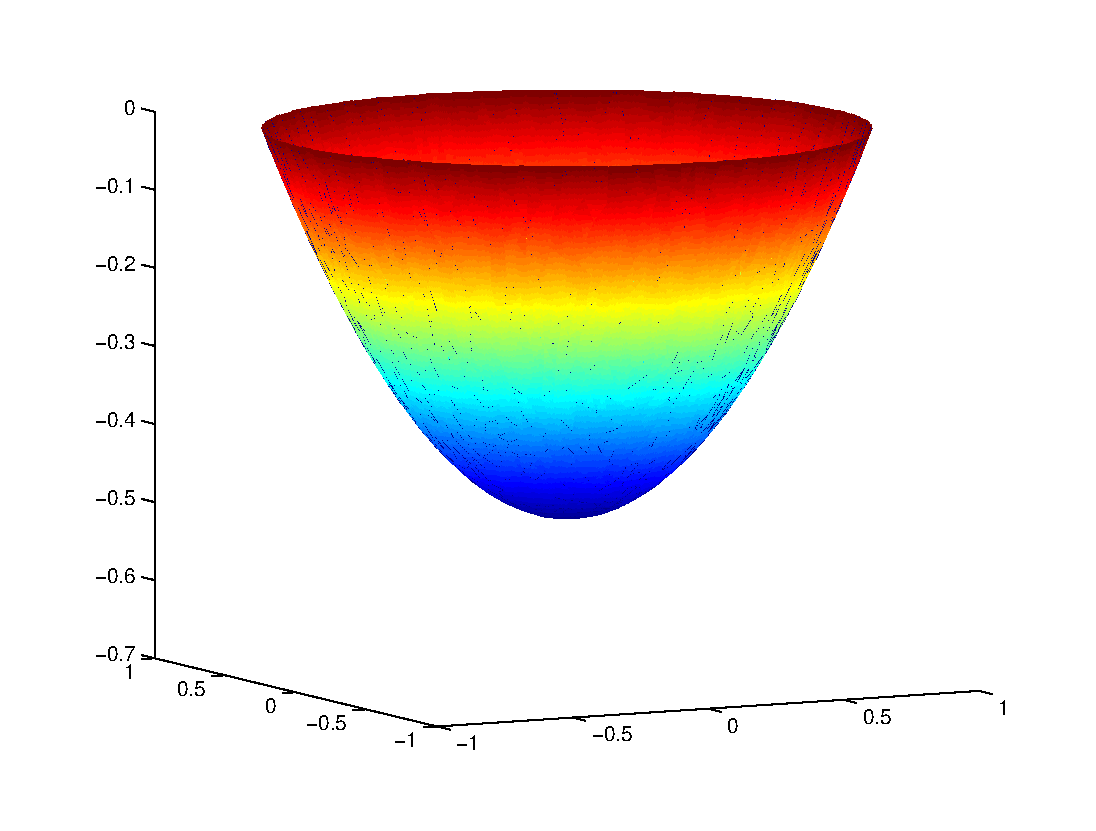
\includegraphics[width=6.25cm]{Abbildungen/bsp_ohne_hindernis.eps}}
\hfill
\subfigure[mit Hindernis: Ebene $z=-0,28$]{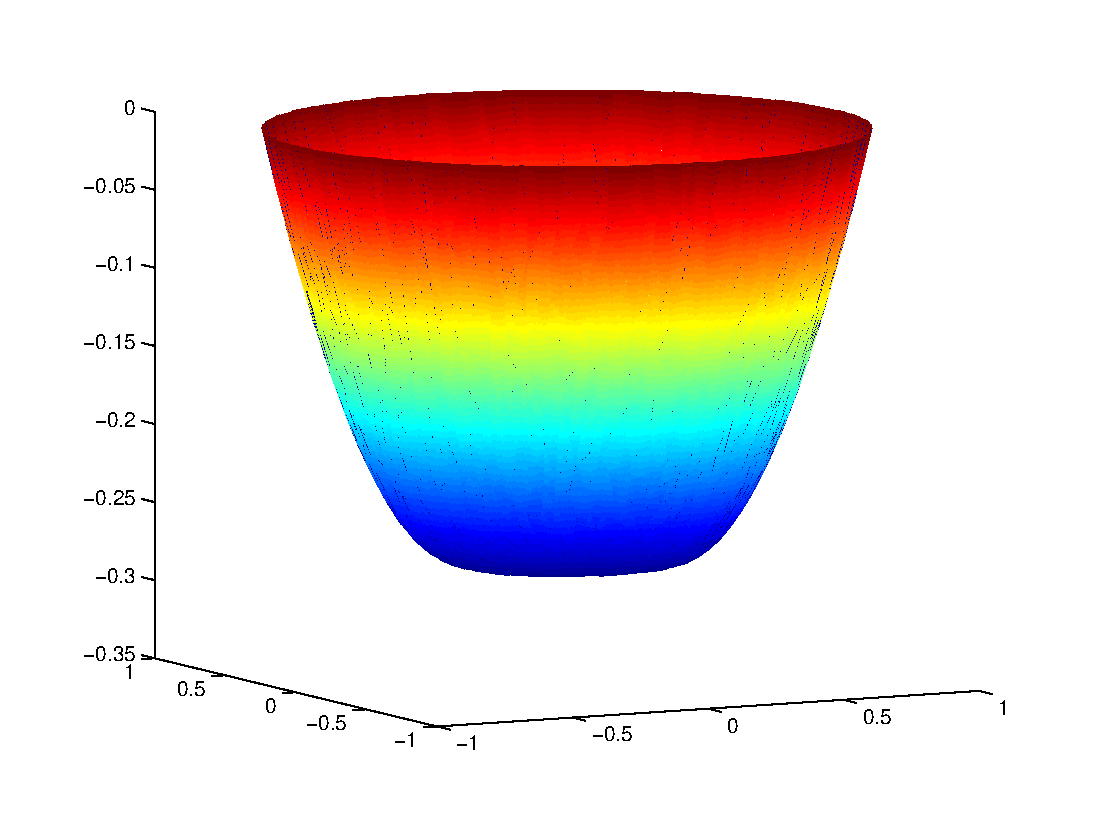
\includegraphics[width=6.25cm]{Abbildungen/bsp_mit_hindernis.eps}}
\end{center}
\caption{Auslenkung einer eingespannten Membran unter Einwirkung einer vertikalen Lastfunktion $f$\label{abb:1.1}}
\end{figure}


Nachdem wir in Kapitel \ref{kap:4} einen hierarchischen a posteriori Fehlerschätzer für das Modellproblem \eqref{eq:1.1} untersucht haben, wollen wir diesen auf Kontaktprobleme übertragen. Für residuale a posteriori Fehlerschätzer sind diese bereits in der Literatur (vgl. z.B. \cite{CarWri}, \cite{WriggersContact} und \cite{HanJoh}) vielfältig untersucht worden. Daher wollen wir ein Kontaktproblem für den in dieser Arbeit eingeführten hierarchischen Fehlerschätzer untersuchen.

Kontaktprobleme sind Probleme aus der Strukturmechanik und stellen eine Anwendung von partiellen Differentialgleichungen unter Nebenbedingung (nämlich der Kontaktbedingung) dar. Wir werden uns in dieser Arbeit mit einem vereinfachten Kontaktproblem, dem \textit{\idx{Signorini-Kontakt}problem} beschäftigen, d.h. es gibt keine Reibungskräfte auf der Kontaktfläche. Außerdem werden wir von einem linear elastischen Fall ausgehen, d.h. das Hooke'sche Gesetz gilt. Die Lösung eines Kontaktproblems kann wie oben eindeutig (vgl. Kapitel \ref{kap:3.2}) durch die Minimierung des Energiefunktionals
\begin{align}\label{eq:1.2}
	\mcal J (\bs v) = \frac 12 \int_\Omega \bs \sigma (\bs v):\bs \eps(\bs v) \, d\Omega - \int_\Omega \bs b\cdot \bs v \, d\Omega - \int_{\Gamma} \bs t\cdot \bs v \, d\Gamma 
\end{align}
über $\mscr K$ berechnet werden, wobei die Menge $\mscr K$ diejenigen Verschiebungsfelder $\bs v$ enthält, die die Kontaktbedingung $\bs v \cdot\bs n - g \le 0$ erfüllen. Die Funktion $g$ gibt hierbei die Lücke zwischen den beiden Körpern an und wird daher auch als \textit{\idx{Gap-Funktion}} bezeichnet. Diese  stellt für Problem \eqref{eq:1.2} also das Hindernis dar, wie zuvor $\psi$ für \eqref{eq:1.1}. In Kapitel \ref{kap:4.4} werden dann die Übertragungen der Konzepte des Fehlerschätzers für Problem \eqref{eq:1.1} beschrieben. Weiter stellt $\bs \sigma$ die Spannung, $\bs \eps$ die Verzerrung und $\bs b$ die Volumenlast (z.B. Gewichtskraft) im vorliegenden Körper dar, der durch $\Omega$ beschriebenen wird. Die Funktion $\bs t$ beschreibt eine Oberflächenlast, die auf den Körper wirkt.

Zunächst werden wir jedoch in Kapitel \ref{kap:3} zeigen, dass die beiden Probleme \eqref{eq:1.1} und \eqref{eq:1.2} grundlegend auf dieselben Variationsungleichungen führen und die Existenz einer eindeutigen Lösung für solch eine Variationsungleichung, und damit auch für die jeweiligen Probleme, zeigen.

Zuvor werden in Kapitel \ref{kap:2}  grundlegende Konzepte zu Hilberträumen, Variationsrechnung, adaptive Verfeinerungsstrategien und der Strukturmechanik eingeführt. Weitere Resultate, die in der vorliegenden Arbeit verwendet werden und nicht in Kapitel \ref{kap:2} aufgeführt sind, können in Anhang \ref{anhang:A} (Funktionalanalysis), \ref{anhang:B} (Optimierung) und \ref{anhang:C} (Tensorrechnung) nachgeschlagen werden.

Die Lösungsverfahren für die adaptive Verfeinerung der Hindernis- bzw. Kontaktprobleme werden in Matlab implementiert und die wichtigsten Vorgehensweisen hierfür in Kapitel \ref{kap:5} beschrieben. Der Quellcode ist im Detail im Anhang \ref{anhang:D} einzusehen.

In Kapitel \ref{kap:6} werden wir abschließend mehrere Beispiele für Hindernis- bzw. Kontaktprobleme präsentieren, welche die Resultate aus Kapitel \ref{kap:4} untermauern.



\newpage

%%% Local Variables: 
%%% mode: latex
%%% TeX-master: "Skript"
%%% End: 

\newchapter{Grundlagen}
\label{kap:2}

In diesem Kapitel wollen wir uns mit grundlegender Theorie beschäftigen, die nicht im Anhang aufgeführt, zum Verständnis von den darauffolgenden Kapiteln jedoch notwendig ist.

Dieses Kapitel basiert auf \cite{BraeFEM}, \cite{StarkePDE}, \cite{EPS}, \cite{Walker}, \cite{AltKonti}.


\section{Hilberträume}
\label{kap:2.1}


Wir benötigen für die Variationsrechnung Hilberträume und wollen uns daher in diesem Kapitel mit wichtigen Eigenschaften solcher Räume im Allgemeinen beschäftigen. Zunächst führen wir ein, was wir unter einem Hilbertraum verstehen.


\begin{defi}\label{def:2.1}
Ein \textit{\idx{Hilbertraum}} ist ein reeller oder komplexer Vektorraum $H$ mit Skalarprodukt $(\cdot, \cdot)_H$, der vollständig bzgl. der durch das Skalarprodukt induzierten Norm, $\norm v_H^2 \coloneqq{(v,v)_H}$ für alle $v \in H$, ist, d.h. in dem jede Cauchy-Folge konvergiert.
\end{defi}


\begin{bsp*}
Es sei $H = \R^n$ und $(\cdot,\cdot)_H : \R^n\times \R^n \ra \R$ definiert durch das Standartskalarprodukt. Dann konvergiert jede \idx{Cauchy-Folge} in $H$ bzgl. der durch $(\cdot,\cdot)_H$ induzierten (euklidischen) Norm (vgl. \cite{Ana2}, metrische Räume) und damit ist $H$ ein Hilbertraum.
\end{bsp*}


Wir wollen die im Folgenden aufgeführten Eigenschaften später auf weniger triviale Räume anwenden, vor allem den Funktionenraum $H^1_0(\Omega)$ (s. Anhang \ref{anhang:A} Sobolev-Räume\index{Sobolev-Raum}). Um alle Aussagen auch allgemein verwenden zu können, sei in diesem Kapitel $H$ ein reeller Hlbertraum mit Skalarprodukt $(\cdot,\cdot)_H$ und der dazu induzierten Norm $\norm v_H^2 = (v,v)_H$ für alle $v \in H$.


\begin{bem*}
Für alle $v,w \in H$ gilt die \idx{Cauchy-Schwarz'sche Ungleichung}
\[
	(v,w)_H \le \norm v_H \, \norm w_H \, .
\]
\end{bem*}


Da wir uns in dieser Arbeit mit Variationsproblemen über konvexen abgeschlossenen Mengen beschäftigen werden, sammeln wir zunächst einige Aussagen bzgl. dieser Mengen.


\begin{satz}[\idx{Approximationssatz}]\label{satz:2.2}
Es sei $\emptyset\neq M\subset H$ konvex und abgeschlossen. Dann existiert für alle $v\in H$ ein $m_v\in M$ mit
\[ 
  	\norm{v-m_v}=\dist(v,M)\coloneqq \inf_{w\in M}\norm{v-w}\, .
\]
Wir nennen $P_M:H\ra M$ mit $v\mapsto m_v$ die \idx{Projektionen} auf $M$.
\end{satz}

\begin{proof}
Der Beweis ist in \cite{Walker} Kapitel 7.1 Satz 7.2 zu finden.
\end{proof}


\begin{satz}[Charakterisierung der Projektionen]\label{satz:2.3}
$\emptyset\neq M\subset H$ sei abgeschlossen und konvex und $v\in H$. Dann gilt:
\[ 
  	m_0=P_M(v)\quad\Longleftrightarrow\quad (m-m_0, v-m_0)_H\leq0 
\]
für alle $m\in M$.
\end{satz}

\begin{proof}
 Es sei o.B.d.A. $0\in M$ und $m_0=0$.
 
  "`$\Rightarrow$"' Wegen $0=P_M(x)$ muss $\norm{v-tm}_H\geq\norm v_H$ für $m\in M$ und $0\leq t\leq1$ sein. Dann ist
\begin{align*}
    	 \norm v^2_H\leq\norm v^2_H-2t(v, m)_H+t^2\norm m^2_H
	\ \lra \ 0 \le - 2t (v,m)_H + \underbrace{t^2 \norm m_H^2}_{\ge 0} \, .
 \end{align*}
Damit ist $2(v, m)_H\leq0$.
 
 "`$\La$"' Für alle $m\in M$ ist $(v, m)_H\leq0$. Es folgt
\[ 
	\norm v^2_H\leq\norm v^2_H+\norm m^2-2(v,m)_H=\norm{v-m}^2_H\, . 
\]
Wegen $0\in M$ ist $\dist(v,M)=\norm v^2_H$ und damit $0=P_M(v)$.
\end{proof}


\begin{satz}\label{satz:2.4}
Es sei $\emptyset \not = M \subset H$ konvex und abgeschlossen. Dann gilt:
\[
	\norm{P_M(v)-P_M(w)}_H \le \norm{v-w}_H \quad \forall \, v,w \in H \, .
\]
\end{satz}

\begin{proof}
Da $P_M(v), P_M(w) \in M$ für alle $v,w \in H$ ist, folgt aus Satz \ref{satz:2.3}
\begin{align}\label{eq:2.1}
	(P_M(w)-P_M(v),v-P_M(v))_H  \le 0 \, , \\
	(P_M(v)-P_M(w),w-P_M(w))_H \le 0 \, .\label{eq:2.2}
\end{align}
Addieren wir \eqref{eq:2.1} und \eqref{eq:2.2}, so erhalten wir
\begin{align*}
	0 &\ge (P_M(w)-P_M(v),v-P_M(v))_H + (P_M(v)-P_M(w),w-P_M(w))_H \\
	& = (P_M(w)-P_M(v),v-w+P_M(w)-P_M(v))_H \\
	& = \norm{P_M(w)-P_M(v)}_H^2-(P_M(w)-P_M(v),w-v)_H \\
	&\!\!\!\: \stackrel{\scriptsize \text{C.S.}}\ge \norm{P_M(w)-P_M(v)}_H^2 - \norm{P_M(w)-P_M(v)}_H \, \norm{w-v}_H \, .
\end{align*}
Nach Umstellen der Ungleichung folgt die Behauptung.
\end{proof}


\begin{defi}\label{def:2.5}
Es sei $\emptyset\neq M\subset H$ und wir definieren das \textit{{orthogonale Komplement}}\index{orthogonales~Komplement} von $M$ durch
\[
	M^\perp\coloneqq\{v\in H\with v\perp M\}\coloneqq\{v\in H\with (v, m)_H=0\;\fa\,  m\in M\}\, .
\]
\end{defi}


\begin{satz}\label{satz:2.6}
 Es sei $M$ ein abgeschlossener Untervektorraum von $H$. Dann ist
  \[
  	H=M\oplus M^\perp\, , 
  \]
  d.h. jedes $v\in M$ hat eine eindeutige Zerlegung $v=v_M+v_{M^\perp}$ mit $v_M\in M$ und $v_{M^\perp}\in M^\perp$.
\end{satz}

\begin{proof}
Der Beweis findet sich in \cite{Walker} Kapitel 7.1 Theorem 7.6.
\end{proof}


\begin{kor}\label{kor:2.6}
Es sei $\emptyset \not = M \subset H$   ein Untervektorraum. Dann ist $\bar M = H$ genau dann, wenn $M^\perp = \{0\}$ ist.
\end{kor}

\begin{proof}
Man kann zeigen, dass $\overline{\spn M} = (M^\perp)^\perp =: M^{\perp\perp}$ ist und dann unter Verwendung von Satz \ref{satz:2.6} die Behauptung folgern. Den kompletten Beweis können wir in \cite{Walker} Kapitel 7.1 Korollar 7.7 (iii) einsehen.
\end{proof}



\section{Variationsformulierung}
\label{kap:2.2}


Bevor wir uns mit Variationsproblemen auf konvexen Teilmengen eines Hilbertraumes beschäftigen, wollen wir die Variationsrechnung an einem einfachen Modellproblem ohne Nebenbedingung beschreiben.

Wir betrachten als Modellproblem die Auslenkung $u: \Omega \ra \R$ einer in $\Omega \subset \R^d$ eingespannten Membran unter Krafteinwirkung $f$. Mathematisch beschrieben wird dies durch das  \textit{\idx{Dirichlet-Problem}}
\begin{subequations}\label{eq:2.1a}
\begin{align}\label{eq:2.1aa}
%\begin{aligned}
	-\Delta u &= f \text{ in } \Omega \, ,\\
	\label{eq:2.1ab}
	u & = g \text{ auf } \partial \Omega \, ,
%\end{aligned}
\end{align}
\end{subequations}
dabei ist $g: \partial \Omega \ra \R$ eine für die Randwerte von $u$ gegebene Funktion.


\begin{notation} 
In der Praxis übliche Dimensionen sind $d = 2,3$. Der Einfachheit halber sei im Folgenden $d = 2$ und $\Omega \subset \R^2$ ein durch ein Polygonzug berandetes Gebiet, den Rand $\partial \Omega$ bezeichnen wir auch mit $\Gamma$.
\end{notation}


\begin{bem*}
Sollte $\Omega$ ein allgemeiner berandetes Gebiet sein, so können wir dieses beliebig genau durch ein polygonales Gebiet approximieren; hierbei entsteht schon bei der Gebietszerlegung ein Fehler.

Diesen Fehler kann man durch Verwendung von \textit{isoparametrischen Elementen}\index{isoparametrisches Element} (vgl. \cite{BraeFEM} Kapitel III, \S2, Isoparametrische Elemente) verringern. Dies soll in dieser Arbeit aber nicht weiter vertieft werden.
\end{bem*}


Es sei $u_0: \Omega \ra \R$ eine für das \idx{Dirichlet-Problem} zulässige Funktion, d.h. die für   \eqref{eq:2.1a} hinreichend regulär ist und für die $u_0 = g$ auf $\Gamma$ gilt. Dann gilt für 
$\tilde u = u-u_0$
\begin{subequations}\label{eq:2.2a}
\begin{align}\label{eq:2.2aa}
	-\Delta \tilde u &= \tilde f \text{ in } \Omega \, ,\\
	\label{eq:2.2ab}
	\tilde u & = 0 \text{ auf } \Gamma 
\end{align}
\end{subequations}
mit $\tilde f = f-\Delta u_0$. Also reicht es aus, sich auf das \textit{homogene Dirichlet-Problem}\index{Dirichlet-Problem!homogenes} \eqref{eq:2.2a} zu beschränken. Im Folgenden betrachten wir somit \eqref{eq:2.1a} mit $g \equiv 0$.

Mit $H^1_0 (\Omega)$ bezeichnen wir, wie in Bemerkung \ref{bem:A.8} beschrieben, den Raum der einmal schwach differenzierbaren Funktionen, die am Rand $\Gamma$ verschwinden im Sinne der Spur.



\begin{itemize}
\item für $v \in H^1_0(\Omega)$ gilt dann mit \eqref{eq:2.1a}
\begin{align*}
	\int_\Omega -\Delta u \cdot v \, dx = \int_\Omega f v \, dx \, .
\end{align*}
Betrachte also \eqref{eq:2.1a} im Mittel über das ganze Gebiet $\Omega$. Durch Anwenden der 1. Green'schen Formel (bzw. Satz von Gauß) ergibt sich
\begin{align}
\notag	& \int_\Omega \nabla u \cdot \nabla v \, dx -\underbrace{\int_\Gamma v \partial_\nu u \, ds}_{=0, \text{ da } v|_\Gamma = 0} = \int_\Omega f v \, dx \, \\
\label{eq:2.3}	\Llra & \quad \qquad \int_\Omega \nabla u \cdot \nabla v \, dx =\int_\Omega f v \, dx
\end{align}
\item kurz geschrieben ist \eqref{eq:2.3} mit der Notation aus Satz \ref{satz:A.5} (b) 
\[
	(\nabla u, \nabla v)_0 = (f,v)_0 \, .
\]
\item wir definieren die Bilinearform $a: (H^1_0(\Omega))^2 \ra \R, a(u,v) := (\nabla u, \nabla v)_0$ und $(f,v):=(f,v)_0$.
\begin{defi}
Eine Funktion $u \in H^1_0(\Omega)$ heißt \textit{\idx{schwache Lösung}} vom \idx{homogenen Dirichlet-Problem}
\begin{align}\label{eq:DP}\tag{DP}
\begin{aligned}
	-\Delta  u &=  f \text{ in } \Omega \, ,\\
	 u & = 0 \text{ auf } \Gamma \, ,
\end{aligned}
\end{align}
wenn die Gleichung
\begin{align}\label{eq:2.4}
	a(u,v) = (f,v)\quad \forall \, v \in H^1_0(\Omega) 
\end{align}
gilt.
\end{defi}
\item Wir betrachten im folgenden alle Hilberträume über $\R$.
\item Frage nach der Existenz und Eindeutigkeit einer schwachen Lösung für \eqref{eq:DP} $\Ra$ hierfür wird ein Hilbertraum benötigt (nachher im Beweis ersichtlich) $\ra$ Lösung liefert der Satz von Lax-Milgram.
\item zuvor noch eine Definition.
\begin{defi}
Sei $H$ ein Hilbertraum. Die Bilinearform  $a : H\times H \ra \R$ heißt \textit{stetig}\index{Bilinearform!stetig}, falls mit einem $c>0$
\[
	\abs{a(u,v)} \le c \, \norm{u}_H   \norm{v}_H \quad \forall \, u,v \in H
\]
gilt. Sie heißt $H$-\textit{elliptisch} (oder kurz \textit{elliptisch} oder \textit{koerziv})\index{Bilinearform!koerziv}\index{Bilinearform!elliptisch}, falls es ein $\alpha > 0$ gibt, so dass
\[
	a(v,v) \ge \alpha \, \norm{v}_H^2 \quad \forall \, v \in H 
\]
gilt.
\end{defi}

\item Bevor Existenz der Lösung gezeigt, betrachte Funktional $J(v) = \frac 1 2 a(v,v)-F(v)$ genauer

\item 
\begin{lemma}\label{lem:2.3}
Es sei $H$ ein Hilbertraum. Das Funktional
\[
	J: H \ra \R \, , \quad J(v) := \frac 1 2 a(v,v) - F(v) \, ,
\]
wobei $a: H\times H \ra \R$ eine stetige bilineare koerzive und $F: H\ra \R$ eine lineare Abbildung ist, ist konvex.
\end{lemma}

\begin{proof}
Es seien $u,v \in H$, dann gilt $u + t(v-u) = (1-t)u + tv \in H$ (dies gilt auch, wenn wir den Satz auf eine konvexe Teilmenge $M \subset H$ beschränken). Damit folgt mit $t \in [0,1]$
\begin{align*}
	J((1-t)u+tv)  = & \frac 1 2 a((1-t)u+tv,(1-t)u+tv) - F((1-t)u+tv) \\
	= &(1-t) \, J(u) + t \, J(v) +  \frac 1 2 a((1-t)u+tv,(1-t)u+tv) \\
	 & - \frac 1 2(1-t) \, a(u,u)-\frac 1 2 t \, a(v,v) \\
	= & (1-t) \, J(u) + t \, J(v)  + \frac 1 2 a(u,u) + t \, a(u,v-u)  \\
	&+ \frac {t^2} 2 a(v-u,v-u) - \frac 12 (1-t)\, a(u,u) -\frac 1 2 t \, a(v,v) \\
	= & (1-t) \, J(u) + t \, J(v) + \frac {t^2} 2 a(v-u,v-u)  \\
	 &\underbrace{+ t \, a(u,v)  - \frac 12 t\, a(u,u) -\frac 1 2 t \, a(v,v) }_{=  -\frac 1 2 t\, a(v-u,v-u)}\\
	= &  (1-t) \, J(u) + t \, J(v) - \frac {1} 2 \underbrace{t \, (1-t)}_{\ge 0} \,\underbrace{ a(v-u,v-u) }_{\ge \alpha  \norm{v-u}_H^2 \ge 0} \\
	\le &   (1-t) \, J(u) + t \, J(v) \, .% \qedhere
\end{align*}
Daraus folgt die Behauptung.
\end{proof}
\item \begin{lemma} \label{lem:2.4}
Sei $H$ ein Hilbertraum. Das Funktional $J: H \ra \R, J(v) =\frac 1 2 a(v,v)-F(v)$ aus Lemma \ref{lem:2.3} ist Gâteaux-differenzierbar $($s. Definition \ref{def:Gateaux-Ableitung}$)$.
\end{lemma}

\begin{proof}
Wir rechnen einfach nach, dass der Grenzwert des Differenzenquotienten existiert und verwenden dabei die Bilinearität von $a$ und Linearität von $F$. Seien $u,v \in H$, dann gilt
\begin{align*}
	\mscr D_v J(u) & = \lim_{t\ra 0} \frac{J(u+tv)-J(u)}t \\ 
	&= \lim_{t\ra 0} \frac{J(u) + t \, (a(u,v)-F(v)) + \frac {t^2}2 a(v,v)-J(u)}t \\
	& =  \lim_{t\ra 0}  (a(u,v)-F(v)) + \frac {t}2 a(v,v) \\
	& = a(u,v)-F(v) < \infty\, ,
\end{align*}
da $a$ und $F$ jeweils stetig sind und daher durch $\norm u_H,\norm v_H$ beschränkt sind. Damit folgt die Behauptung.
\end{proof}
\item 
\begin{theorem}\label{theorem:Lax-Milgram}\textnormal{(Lax-Milgram)}
Es sei $H$ ein Hilbertraum und  $a : H \times H \ra \R$ eine symmetrische, in $H$ stetige, koerzive Bilinearform. Weiter sei $F:H\ra \R$ ein stetiges lineares Funktional, d.h.
\[
	\abs{F(v)} \le c \, \norm{v}_H \quad \forall \, v \in H
\]
mit einer Konstante $c >0$. Dann gibt es eine eindeutige Lösung $u \in H$, für die
\[
	a(u,v) = F(v) \quad \forall \, v \in H \, .
\]
gilt. Diese minimiert den Ausdruck
\[
	J(v) = \frac 1 2 a(v,v) - F(v)
\]
unter allen $v \in H$.
\end{theorem}

\begin{proof}
(i) Zunächst zeigen wir die Äquivalenz der beiden oberen Probleme.

"`$\Ra$"' Es sei $u\in H$, so dass $a(u,v) = F(v) \, \forall \, v \in H$. Für $t>0$ und $v\in H$ gilt dann
\begin{align*}
	J(u+tv) & = \frac 1 2 a(u+tv,u+tv) -F(u+tv) \\
	& = \frac 1 2 a(u,u) + t \, a(u,v) + \frac {t^2} 2 a(v,v)-F(u)-t \, F(v) \\
	& = \frac 1 2 a(u,u)-F(u) + t\, (\underbrace{a(u,v)-F(v)}_{=0}) + \frac{t^2}2 \underbrace{a(v,v)}_{\parbox{1.2cm}{\scriptsize$\ge 0$, da $a$ koerziv}} \\
	& > \frac 1 2 a(u,u) - F(u) = J(u) \, ,
\end{align*}
also ist $u = \arg\min\limits_{v\in H} J(v)$.

"`$\La$"' Es sei $u \in H$ das Minimum von dem Problem
\[
	\min_{v\in H} J(v) = \frac 1 2 a(v,v) -F(v) \, .
\]
Da $J:H\ra \R$ nach Lemma \ref{lem:2.3} ein konvexes Funktional ist und $J$ nach Lemma \ref{lem:2.4} Gâteaux-differenzierbar, gilt mit Satz \ref{satz:A.10} für alle $v \in H$
\begin{align*}
	0& = \mscr D_vJ(u) = \frac d{dt} J(u+tv)\Big|_{t=0} \\
	& = \frac d{dt}(J(u) + t \, (a(u,v)-F(v))+\frac{t^2}2 a(v,v))\Big|_{t=0} \\
	& = a(u,v)-F(v) + t \, a(v,v) \Big|_{t=0} = a(u,v)-F(v)
\end{align*}
(ii) Eindeutigkeit: Es seien $u,\tilde u \in H$ Lösungen der Variationsungleichung, d.h.
\begin{align*}
	a(u,v) = F(v) \, \wedge \, a(\tilde u,v) = F(v) \quad \forall \, v \in H \, .
\end{align*}
Damit folgt durch Subtraktion der beiden Gleichungen für alle $v \in H$
\begin{align}\label{eq:2.5}
	a(u,v) = a(\tilde u,v) \Llra a(u-\tilde u,v) = 0 \, .
\end{align}
Da $H$ ein Vektorraum ist, gilt auch $u-\tilde u \in H$. Ersetzen wir also in \eqref{eq:2.5} $v = u-\tilde u$, dann ergibt sich
\begin{align*}
	&0 = a(u-\tilde u,u-\tilde u) \stackrel{\scriptsize a\text{ koerziv}}\ge \underbrace{\alpha}_{>0} \norm{u-\tilde u}_H^2 \ge 0 
	\lra\norm{u-\tilde u}_H^2 = 0 \, ,
\end{align*}
also folgt $u = \tilde u$.

(iii) Existenz: Die Existenz einer Lösung weisen wir über das Funktional nach.
\begin{align*}
	J(v) & = \frac 1 2 a(v,v)-F(v) \stackrel[\scriptsize F \text{ linear}]{\scriptsize a \text{ koerziv}}\ge \frac 1 2 \alpha \norm v_H^2 - c \norm v_H \\
	& = \frac 1 2 \alpha \(\norm v_H^2 - \frac{2c}\alpha \norm v_H\) = \frac 1 2 \alpha\(\norm v_H - \frac c\alpha\)^2 - \frac {c^2}{2\alpha} \\
	& \ge - \frac{c^2}{2\alpha}
\end{align*}
Folglich ist $J$ nach unten beschränkt. Sei $\eta := \inf \{J(v)\with v \in H\}$ und $(v_n)_{n\in\N}$ eine Folge mit $J(v_n) \ra\eta$ für $n\ra \infty$. Dann folgt mit der Koerzivität von $a$
\begin{align*}
	\alpha \norm{v_n-v_m}^2_H  \le & a(v_n-v_m,v_n-v_m) \\
	 = &a(v_n,v_n)+a(v_m,v_m)-a(v_n,v_m)-a(v_m,v_n) \\
	=& 2a(v_n,v_n)+2a(v_m,v_m) \underbrace{-a(v_n,v_n+v_m)-a(v_m,v_n+v_m)}_{=-a(v_n+v_m,v_n+v_m)} \\
	=& 2a(v_n,v_n)-4F(v_n)+2a(v_m,v_m)-4F(v_m) \\
	& -a(v_n+v_m,v_n+v_m)+4F(v_n+v_m) \\
	= & 4 J(v_n) + 4J(v_m) - 4 a\(\frac{v_n+v_m}2,\frac{v_n+v_m}2\)+8F\(\frac{v_n+v_m}2\) \\
	= & 4 J(v_n) + 4J(v_m) - 8 J\(\frac{v_n+v_m}2\) \\
	\le &4 J(v_n) + 4J(v_m) - 8\eta  \xrightarrow[n,m\ra\infty]{} 4\eta+4\eta-8\eta = 0 \, ,
\end{align*}
d.h. $(v_n)_{n\in \N}$ ist eine Cauchy-Folge. Da $H$ ein Hilbertraum ist, gilt somit: $\exists \, u \in H : v_n \xrightarrow[n\ra \infty]{} u$ mit $J(u) = \eta$.
\end{proof}

\item
\begin{satz}\textnormal{(\idx{Poincaré-Friedrich-Ungleichung})}\label{satz:2.13}
Es sei $\Omega$ in einem $d$-dimensionalen Würfel der Kantenlänge $s>0$ enthalten. Dann gilt
\[
	\norm v_0 \le s \norm{\nabla v}_0 \quad \forall \, v \in H^1_0(\Omega) \, ,
\]
wobei $\norm\cdot_0$ die durch das Skalarprodukt $(\cdot,\cdot)_0$ induzierte Norm ist.
\end{satz}

\begin{proof}
Der Beweis ist in \cite{BraeFEM} Kapitel II, \S1 Sobolev-Räume, Satz 1.5 oder \cite{StarkePDE} Satz 1.5 zu finden.
\end{proof}

\begin{bem}
Für die Gültigkeit der Poincaré-Friedrich-Ungleichung, muss $v$ nicht auf ganz $\Gamma$ gleich Null sein, sondern es reicht aus, dass
\[
	v \in H^1_{\Gamma_u} (\Omega)\coloneqq \{v \in H^1(\Omega) \mid v = 0 \text{ auf } \Gamma_u\}
\]
ist mit $\Gamma_u \subset \Gamma$ und einem Maß $\mu (\Gamma_u) \not = 0$ (vgl. \cite{BraeFEM} Kapitel II, \S1, Bemerkung 1.6).
\end{bem}

\item Greifen wieder die Frage auf, ob das Problem \eqref{eq:2.4} mit $a:(H^1_0(\Omega))^2\ra \R, a(u,v) = (\nabla u,\nabla v)_0$ und $F:H^1_0(\Omega) \ra \R, F(v) := (f,v)$ eine eindeutige Lösung hat.
\item Kann nun mit Theorem \ref{theorem:Lax-Milgram} beantwortet werden. Es seien $u,v \in H^1_0(\Omega)$, dann gilt
\begin{align*}
	 a(v,v) = & \int_\Omega \nabla v \nabla v \, dx = \norm{\nabla v}_0^2  \\
	\ge& \frac{s^2+1}{(1+s)^2}\norm{\nabla v}_0^2  \stackrel{\scriptsize \text{Satz \ref{satz:2.13}}}\ge \frac 1{(1+s)^2} (\norm v_0^2 + \norm{\nabla v}_0^2) \\
	= & \frac 1{(1+s)^2} \norm v_1^2 \, .
\end{align*}
Damit ist $a$ mit $\alpha :=  \frac 1{(1+s)^2}$ koerziv. Weiter rechnen wir nach:
\begin{align*}
	\abs{a(u,v)} = & \Abs{\int_\Omega \nabla u \nabla v \, dx} \le \sum_{i = 1}^d \int_\Omega\abs{\partial_i u}\abs{\partial_i v} \, dx \\
	\stackrel{\scriptsize\text{CS}}\le & \sum_{i = 1}^d \(\int_\Omega \abs{\partial_i u}^2 \, dx\)^{\frac 12} \(\int_\Omega \abs{\partial_i v}^2 \, dx\)^{\frac 12} \\
	\le & \(\sum_{i = 1}^d \int_\Omega \abs{\partial_i u}^2 \, dx\)^{\frac 12} \(\sum_{i=1}^d\int_\Omega \abs{\partial_i v}^2 \, dx\)^{\frac 12} \\
	\le & \( \int_\Omega \abs{\nabla u}^2 \, dx + \int_\Omega u^2 \, dx\)^{\frac 12} \(\int_\Omega \abs{\nabla v}^2 \, dx+\int_\Omega v^2\, dx\)^{\frac 12} \\
	= & \norm u_1 \, \norm v_1 \, ,
\end{align*}
d.h.  $a$ ist stetig mit $c := 1$. Die Symmetrie von $a$ ist trivial, also bleibt nur noch die Stetigkeit von $F$ zu zeigen. Es sei $v \in H^1_0(\Omega)$, dann gilt
\begin{align*}
	\abs{F(v)} &= \abs{(f,v)} =  \Abs{\int_\Omega fv \, dx} \stackrel{\scriptsize\text{CS}}\le\( \int_\Omega \abs{f}^2 \,dx\)^{\frac 12} \( \int_\Omega \abs v^2 \, dx\)^{\frac 12} \\
	&\le  c \, \( \int_\Omega \abs{\nabla v}^2 +  \abs v^2 \, dx\)^{\frac 12} = c \, \norm v_1
\end{align*}
mit $0<c := \int_\Omega \abs f^2 \, dx < \infty$, wenn $f \in L_2(\Omega)$ ist. Damit ist $F$ ein stetiges lineares Funktional und somit existiert nach Theorem \ref{theorem:Lax-Milgram} eine eindeutige Lösung $u \in H^1_0(\Omega)$ für die schwache Formulierung des homogenen Dirichlet-Problems. 

\item Weiter minimiert die Lösung $u \in H^1_0(\Omega)$ das Funktional
\begin{align*}
	J(v) = \frac 12 \int_\Omega \nabla v\nabla v \, dx - \int_\Omega fv \, dx \, ,
\end{align*}
welches die gespeicherte Energie der durch die Kraft $f$ belasteten Membran $\Omega$ beschreibt.

\item \begin{bem*}
Die Stetigkeit vom Funktional $F$ zeigt, welche Eigenschaft die Kraft $f$ aus dem Dirichlet-Problem wenigstens quadratisch integrierbar sein muss, damit es eine schwache Lösung geben kann.
\end{bem*}

\item \begin{bem*}
\begin{enumerate}[(a)]
\item Mit $H'$ bezeichnen wir den Dualraum zu einem Hilbertraum $H$.
\item Den Dualraum zu $H^1(\Omega)$ bezeichnen wir mit $H^{-1}(\Omega)$.
\end{enumerate}
\end{bem*}
\item Hier noch eine Folgerung aus dem Satz von Lax-Milgram:
\begin{satz}[\idx{Riesz'scher Darstellungssatz}]\label{satz:2.14}
Es sei $H$ ein Hilbertraum mit einem Skalarprodukt $(\cdot,\cdot)_H$. Es sei $F \in H'$, dann existiert genau ein $u \in H$, so dass
\[
	(u,v)_H = F(v) \quad \forall \, v \in H \, .
\]
\end{satz}

\begin{proof}
Dies ist eine direkte Folgerung aus dem Theorem \ref{theorem:Lax-Milgram}. Die Abbildung $(\cdot,\cdot)_H:H\times H \ra \R$ ist als Skalarprodukt bilinear, symmetrisch und positiv definit, damit auch bzgl. der auf $H$ durch das Skalarprodukt induzierten Norm $\norm v_H := \sqrt{(v,v)_H}$, koerziv. $F$ ist als Element des Dualraumes $H'$ eine lineare stetige Abbildung $F:H\ra\R$ und damit folgt mit $a(\cdot,\cdot) :=(\cdot,\cdot)_H$ aus dem Theorem von Lax-Milgram die Behauptung.
\end{proof}

\item \begin{kor}\label{kor:2.14}
Es sei $H$ ein Hilbertraum mit Skalarprodukt $(\cdot,\cdot)_H$ und $a:H\times H\ra \R$ eine stetige koerzive Bilinearform. Dann existiert genau ein linearer Operator $A : H \ra H$, so dass gilt:
\[
	a(u,v)  = (Au,v)_H \quad \forall \, u , v \in H \, .
\]
\end{kor}

\begin{proof}
Es sei $u\in H$ fest, dann ist $L: H\ra \R, L(v) := a(u,v)$ eine lineare Abbildung, die stetig ist, da
\[
	\abs{L(v)} = \abs{a(u,v)} \stackrel{\scriptsize\text{stetig}}\le c \,  \norm{u}_H \norm v_H  = \tilde c\, \norm v_H
\]
mit $0<\tilde c := c \, \norm u_H$ gilt. Damit folgt nach dem Darstellungssatz von Riesz, dass es ein eindeutiges $l \in H$ gibt, so dass
\[
	a(u,v) = L(v) = (l,v)_H \quad \forall \, v \in H
\]
gilt. Da $u \in H$ jedoch beliebig ist, bleibt zu zeigen, dass es ein eindeutiges $A:H\ra H$ gibt, so dass $Au = l$ ist.

Wir zeigen zunächst mithilfe der Bilinearform $a$, dass $A$ linear ist. Es gilt für $\lambda,\mu \in \R$ und $u,v \in H$
\begin{align*}
	(A(\lambda u + \mu v),w)_H &= a(\lambda u + \mu v, w) = \lambda a(u,w) + \mu a(v,w) \\
	& = \lambda (Au,w)_H + \mu(Av,w)_H \\
	& = (\lambda \, Au+\mu \, Av,w)_H
\end{align*}
für alle $w \in H$. Weiter gilt
\[
	\norm{Au}_H^2 = (Au,Au)_H = a(u,Au) \stackrel{\scriptsize \text{stetig}}\le c \, \norm u_H \norm{Au}_H \, ,
\]
d.h. $\norm{Au}_H \le c \, \norm u_H$ und damit ist nach \cite{Werner} Satz II.1.2 der Operator $A$ stetig.

Betrachten wir den Kern von $A$, so ergibt sich
\begin{align}\label{eq:2.6}
	\ker A := \{ v \in H \with Av = 0\} = \{0\} \, ,
\end{align}
denn
\[
	\alpha \norm v_H^2 \stackrel{\scriptsize \text{koerziv}}\le a(v,v)  = (Av,v)_H \stackrel{\scriptsize \text{CS}}\le \norm{Av}_H \norm v_H 
\]
und damit gilt $\norm{Av}_H \ge \alpha \norm v_H$, d.h. $Av = 0 \Lra v = 0$. Dies impliziert, dass $A$ injektiv ist, denn mit $v_1,v_2\in H, Av_1 = Av_2$ folgt
\[
	0 = Av_1 - Av_2 = A(v_1-v_2) \ \stackrel{\scriptsize\eqref{eq:2.6}}\lra \ v_1 = v_2 \, .
\]
Weiter betrachten wir das Bild von $A$, d.h.
\[
	\im A := \{ v \in H \with \exists \, u \in H : Au = v \} \subset H\, .
\]
Sei $(v_n)_{n \in \N}$ eine Folge mit $v_k \in \im A $ für alle $k \in \N$. Dann folgt, dass für jedes $v_k$ ein $u_k \in H$ existiert mit $A u_k = v_k$. Es gelte, dass $Au_k = v_k \ra v \in H$ geht, dann folgt
\begin{align*}
	\alpha \, \norm{u_n -u_m}_H & \le \norm{A(u_n-u_m)}_H = \norm{Au_n-Au_m}_H \\
	& = \norm{v_n-v_m}_H \xrightarrow[n,m\ra \infty]{} 0 \, ,
\end{align*}
d.h. $(u_n)_{n\in \N} \subset H$ ist eine Cauchy-Folge und konvergiert daher in $H$. Also existiert ein $u \in H$ mit $u_n \ra u$. Mit der Stetigkeit von $A$ folgt dann
\[
	v_n = A u_n \xrightarrow[n\ra \infty]{} Au = v\, ,
\]
d.h. $v \in \im A$ und damit ist $\im A$ abgeschlossen. Wir betrachten nun ein $v \in H$ mit $v \perp \im A \subset H$, dann gilt
\[
	(Au,v)_H = 0 \quad \forall \, u \in H \, .
\]
Damit folgt mit $u = v \in H$ oben eingesetzt
\[
	 0 = (Av,v)_H = a(v,v) \ge \alpha \, \norm v_H^2 \, \lra \, v = 0 \, .
\]
Also besteht der zu $\im A$ orthogonale Raum nur aus dem Nullelement und mit Korollar \ref{kor:2.6} gilt dann $\im A = \overline{\im A} = H$. Damit ist $A$ bijektiv.

Es seien nun $0 \not = l\in H$ sowie $A_1,A_2 \in \mcal L(H,H)$ zwei lineare Operatoren mit $A_1u = l$ und $A_2 u = l$, die nach der obigen Weise konstruiert sind. Dann gilt
\[
	0 = A_1 u - A_2 u = (A_1 - A_2)u \, \lra \, A_1 = A_2 \, , 
\]
da $u \not = 0$ und die Summe zweier bijektiver linearer Operatoren wieder bijektiv ist, also ist ein so konstruierter Operator eindeutig.
\end{proof}
\end{itemize}






\section{Finite Elemente Methode}
\label{kap:2.3}

\begin{itemize}
\item FEM $\ra$ einleitend ansprechen, dass analytische nicht immer lösbar

\item Unter FEM verstehen wir das Galerkin-Verfahren

\item Galerkin-Verfahren bedeutet, wir wollen die Variationsgleichung
\begin{align}\label{eq:2.8}
	a(u,v) = F(v) \quad \forall \, v \in H
\end{align}
auf einem endlich dimensionalen Unterraum $V_h \subset H$ lösen, d.h. finde $u_h \in V_h$, so dass
\begin{align}\label{eq:2.9}
	a(u_h,v_h) = F(v_h) \quad \forall \, v_h \in V_h \, .
\end{align}
\item \begin{satz}
Das "`Galerkin-Problem"' hat eine eindeutige Lösung.
\end{satz}

da $V_h$ als Unterraum von $H$ auch ein Hilbertraum ist und die Eigenschaften von $a, F$ weiterhin erfüllt sind, gilt auch hier der Satz von Lax-Milgram, was die Eindeutigkeit und Existenz einer Lösung sichert.

\item ist $\mcal B_h \coloneqq \{\phi_1,\ldots,\phi_N\}$ eine Basis von $V_h$, dann gilt für $u_h \in V_h$:
\begin{align}\label{eq:2.10}
	\exists! \, \bs\mu \in \R^N :  u_h(x) = \sum_{i = 1}^N \mu_i \,  \phi_i(x) \, .
\end{align}

\item da $F(\cdot),a(u,\cdot)$ linear sind und alle $v_h \in V_h$ analog zu oben darstellbar sind, ist \eqref{eq:2.9} äquivalent zum Problem
\[
	a(u_h,\phi_i) = F(\phi_i) \quad \forall \, i = 1, \ldots,N \, ,
\]
mit $u_h = \sum \mu_i \, \phi_i$ eingesetzt ergibt sich
\[
	a(u_h,\phi_i) = a \Big( \sum_{j = 1}^N \mu_j \,  \phi_j,\phi_i \Big) = \sum_{j = 1}^N \mu_j \, a(\phi_j,\phi_i) \, ,
\]
also
\[
	 \sum_{j = 1}^N \mu_j \, a(\phi_j,\phi_i) = F(\phi_i)\quad \forall \, i = 1, \ldots,N \, .
\]
Damit ergibt sich das LGS
\[
	A \bs \mu = \bs f 
\]
mit $A = [a(\phi_j,\phi_i)]_{i,j=1}^N, \bs \mu = [\mu_i]_{i=1}^N$ und $\bs f = [F(\phi_i)]_{i=1}^N$.

\item \begin{bem}\label{bem:2.17}
Ist die Bilinearform $a$ symmetrisch, so ist es auch die Matrix $A$, denn
\[
	a_{ij} = a(\phi_i,\phi_j) = a(\phi_j,\phi_i)= a_{ji} \, .
\]
Außerdem folgt aus der Koerzivität von $a$, dass  mit $0 \not = v \in \R^N$ gilt
\begin{align*}
	v^T A v & = \sum_{i,j=1}^N v_i a_{ij} v_j  =  \sum_{i=1}^N v_i\sum_{j=1}^N \, a(\phi_i,\phi_j) \, v_j   \\
	& = \sum_{i=1}^N v_i \, a\Big(\phi_i,\sum_{j=1}^Nv_j\phi_j\Big) =  a\Big(\sum_{i=1}^N v_i\phi_i,\sum_{j=1}^Nv_j\phi_j\Big) \\
	& = a(v_h,v_h) \ge \alpha \norm{v_h}^2_H > 0 \, ,
\end{align*}
da $v_h \not = 0$ wegen $v \not = 0$. Damit ist $A$ also positiv definit.
\end{bem}

\item in Ingenieurwissenschaften, insbesondere bei kontinuumsmechanischen Problemen, wird $A$ als Steifigkeitsmatrix bezeichnet.

\item um eine Basis $\mcal B_h$ bzgl. $V_h$ beschreiben zu können, muss das Gebiet $\Omega$ in endliche Elemente zerlegt werden. $V_h$ wird dann bzgl. einer Zerlegung $\mcal T_h$ beschrieben.

\item betrachte im weiteren (wie oben schon angesprochen) $\Omega$ als zweidimensionales Gebiet, das mit einem Polygonzug berandet ist.

\item eine gebräuchliche Zerlegung $\mcal T_h$ kann durch Dreiecke oder auch Vierecke geschehen. Wir wollen hier nur Zerlegungen durch Dreiecke betrachten

\item hierfür führen wir den Begriff der Triangulierung ein (vgl. \cite{BraeFEM} Seite 58 oder \cite{StarkePDE} Seite 19)
\begin{defi}[Triangulierung]
Es sei $\Omega \subset \R^2$ ein durch einen Polygonzug berandetes Gebiet. Dann heißt eine Zerlegung aus Dreiecken
\[
	\mcal T = \{T_1,T_2,\ldots,T_M\}
\]
\textit{\idx{Triangulierung}}, wenn gilt:
\begin{enumerate}[(a)]
\item Für alle Dreiecke $T \in \mcal T$ gilt: $T$ ist abgeschlossen.
\item	Ganz $\Omega$ wird durch alle Dreiecke aus $\mcal T$ überdeckt, d.h. $\bar\Omega = \bigcup_{T\in \mcal T} T$.
\item Der Schnitt zweier Dreiecke $T_i\cap T_j$ mit $i \not = j$ überlappt sich nicht, d.h. $\operatorname{int}(T_i)\cap \operatorname{int}(T_j) = \emptyset$.
\end{enumerate}
Wir nennen eine Triangulierung \textit{konform}\index{Triangulierung!konform} oder \textit{zulässig}\index{Triangulierung!zulässig}, wenn zusätzlich gilt:
\begin{enumerate}[(d)]
\item Für jede Kante $k$ eines Dreiecks $T \in \mcal T$ gilt entweder $k \subset \partial \Omega$ oder $k \subset \widetilde T$ für ein weiteres Dreieck $\widetilde T \in \mcal T$. 
\end{enumerate}
Der Radius des Umkreis eines Dreieckes $T$ wird mit $h$ bezeichnet und beschreibt die Größe eines Dreiecks. Wenn jedes Dreieck $T \in \mcal T$ höchstens einen Radius von $h$ hat, so schreiben wir $\mcal T_h$ statt $\mcal T$.
\end{defi}

\item[Skizze] von einer zulässigen und einer nicht zulässigen Triangulierung (hierbei eine Skizze mit hängenden Knoten machen)

\begin{figure}[h]
\begin{center}
\begin{pspicture}(-3,0)(3,2)
	% zulässige Triangulierung:
	\psline(-3,0)(-3,2)
	\psline(-3,0)(-1,0)
	\psline(-1,0)(-3,2)
	\psline(-3,2)(-1,2)
	\psline(-1,2)(-1,0)
	\psline(-3,0)(-1,2)
	\psline(-3,1)(-2,1)
	\psline(-2,2)(-2,1)
	\psline(-2,2)(-3,1)
	
%	\psline(-2,2)(-1.5,1.5)
%	\psline(-1.5,1.5)(-1,0)

%	\psline(-2.5,1.5)(-3,1)
%	\psline(-2.5,1.5)(-1,2)
	
	% nichtzulässige Triangulierung
	\psline(1,2)(2,1)
	\psline(2,1)(1,0)
	\psline(1,0)(1,2)
	\psline(1,0)(3,0)
	\psline(3,0)(2,1)
	\psline(1,2)(3,2)
	\psline(3,2)(3,0)
	\psdot[dotstyle=o, dotsize=4pt](2,1)
\end{pspicture}
\end{center}
\caption{Zulässige und unzulässige Triangulierung (mit hängendem Knoten)}
\end{figure}

\item \begin{bem}
natürlich auch im $\R^3$ analog mit Tetraedern definierbar
\end{bem}

\item vgl. wieder \cite{BraeFEM} Seite 58
\begin{defi}[(quasi-) uniforme Zerlegung]
Eine Familie von Zerlegungen $\{\mcal T_h\}$ heißt \textit{quasi-uniform}\index{Triangulierung!quasi-uniform}, wenn es eine Zahl $\kappa > 0$ gibt, so dass jedes $T \in \mcal T_h$ einen Kreis vom Radius
\[
	\rho_T \ge \frac{h_T}\kappa
\]
enthält, wobei $h_T$ der Radius des Dreiecks $T$ ist.

Eine Familie von Zerlegungen $\{\mcal T_h\}$ heißt \textit{uniform}\index{Triangulierung!uniform}, wenn es eine Zahl $\kappa > 0$ gibt, so dass jedes $T \in \mcal T_h$ einen Kreis vom Radius
\[
	\rho_T \ge \frac{h}\kappa
\]
enthält, wobei $h := \max_{T \in \mcal T_h} h_T$ ist.
\end{defi}

\item[Skizze] Beispiele für eine quasiuniforme Zerlegung (vgl. \cite{BraeFEM} Seite 59) $\ra$ hier noch was zur Erklärung schreiben, wie im Braess

\begin{figure}[h]
\caption{Beispiele quasiuniformer Zerlegungen}
\end{figure}

\item \begin{bem}
Wie man leicht sehen kann, ist jede uniforme Zerlegung auch quasi-uniform. Umgekehrt gilt dies nicht (s. Abbildung oben).

Allerdings lassen uniforme Zerlegungen keine lokalen Verfeinerungen zu. Da dies für adaptive Verfeinerungsstrategien allerdings ausschlaggebend ist, gehen wir im Folgenden immer von einer quasi-uniformen Zerlegung $\mcal T_h$ aus.
\end{bem}

\item nun wollen wir uns Gedanken über unseren Ansatzraum $V_h$ machen.

\item hierfür gibt es viele Möglichkeiten, vergleiche hierzu auch \cite{BraeFEM} Kapitel II, \S5, Tabelle 2, durch Konstruktion der Elemente

\item wir wollen uns weitestgehend aber nur auf ein Element konzentrieren

\item zuvor hierfür ein wichtiges Resultat; sei noch bemerkt, dass eine Fkt. $u$ auf $\Omega$ bei gegebener Zerlegung eine Eigenschaft stückweise hat, wenn sie auf jedem Element diese Eigenschaft besitzt.
\begin{satz}
Sei $k \ge 1$ und $\Omega\subset \R^2$ ein polygonales Gebiet. Eine stückweise beliebig oft differenzierbare Funktion $v : \bar \Omega \ra \R$ liegt in $H^k(\Omega)$ genau dann, wenn $v \in C^{k-1}(\bar\Omega)$ ist.
\end{satz}

\begin{proof}
Der Beweis ist in \cite{BraeFEM} Kapitel II, \S5, Satz 5.2 zu finden.
\end{proof}

\item dies rechtfertigt, dass für unser Modellproblem \eqref{eq:2.4}, welches für $u,v \in H^1_0(\Omega)$ gestellt ist, auf einer Triangulierung $\mcal T_h$ ein Ansatzraum mit stetigen Funktionen $v \in C^0(\Omega)$ verwendet werden kann, also
\[
	V_h \coloneqq \{v \in C^0(\Omega) \with v|_T \in \mcal P_m \text{ für } T\in \mcal T_h, v|_{\partial \Omega} = 0\} \, ,
\]
wobei $\mcal P_m$ der Raum der Polynome vom Grad $m$ ist.

\item wie diesen Raum $V_h$ aufspannen? $\ra $ die einfachste Möglichkeit solch einen Raum aufzuspannen sind nodale Basisfunktionen
\begin{defi}[\idx{nodale Basisfunktion}]
Zu einem Finiten Element Raum $V_h$ und einer gegebenen Zerlegung $\mcal T_h$ sei eine Menge von Punkten $P$ bekannt mit $\abs P = N$. Die Menge $\mcal B_h = \{\phi_1,\ldots,\phi_N\}$ mit $\phi_i \in \mcal P_m, i = 1,\ldots, N$, heißt \textit{\idx{nodale Basis}} (oder \textit{\idx{Lagrange-Basis}}), wenn
\[
	\phi_i (x_j) = \delta_{ij} = \begin{cases}
							1, &  i = j \\
							0 ,& i \not = j
						\end{cases} %\qquad \forall \,\phi_i \in \mcal B_h, x_j \in P
\]
\end{defi}
für alle $\phi_i \in \mcal B_h$ und $x_j \in P$ gilt.

\item folgende Bemerkung erklärt die Anordnung der in der letzten Definition beschriebenen Punkte $P$ 
\begin{bem}
Sei $m \ge 0$. In einem Dreieck $T$ seien auf $m+1$ Linien $l = 1+2+\ldots+(m+1)$ Punkte $z_1,\ldots,z_l$ angeordnet (s. Skizze). Dann gibt es zu jedem $C^0(T)$ genau ein Polynom $p$ vom Grad $m$ mit der Eigenschaft
\[
	p(z_i) = f(z_i) \quad \forall \, i = 1,\ldots,m \, .
\]

\begin{proof}
Der Beweis steht in \cite{BraeFEM} Kapitel II, \S 5, Bemerkung 5.4.
\end{proof}
\end{bem}

\item[Skizze] Dreiecke für die nodalen Basen (linear, quadratisch, kubisch).

\begin{figure}[h]
\begin{center}
\begin{pspicture}(-3,0)(5,2)
	% lineares Element:
	\psline(-3,0)(-3,2)
	\psline(-3,0)(-1,0)
	\psline(-1,0)(-3,2)
	\psdots(-1,0)(-3,0)(-3,2)
	
	% quadratisches Element:
	\psline(0,0)(0,2)
	\psline(0,0)(2,0)
	\psline(2,0)(0,2)
	\psdots(0,0)(0,2)(2,0)(0,1)(1,1)(1,0)
	
	% kubisches Element:
	\psline(3,0)(3,2)
	\psline(3,0)(5,0)
	\psline(5,0)(3,2)
	\psdots(3,0)(5,0)(3,2)(3,1.3333)(3,0.6667)(3.6667,0)(4.3333,0)(3.6667,0.6667)(3.6667,1.3333)(4.3333,0.6667)
	
\end{pspicture}
\end{center}
\caption{Dreiecke für nodale Basen (linear, quadratisch, kubisch)}
\end{figure}

\item damit lässt sich für $V_h$ mit einem beliebigen Polynomgrad $m$ eine eindeutige nodale Basis finden, die den Raum aufspannt.

\item im weiteren wollen wir lineare Ansatzfunktionen verwenden. Wir bezeichnen, sofern nicht anders beschrieben, also im Folgenden $\mcal S_h$ mit
\[
	\mcal S_h \coloneqq \{v \in C^0(\Omega) \with v|_T \in \mcal P_1 \text{ für } T\in \mcal T_h, v|_{\partial \Omega} = 0\} \, .
\]

\item das Galerkin-Verfahren mit dem Ansatzraum $\mcal S_h$ wird Finite-Elemente-Methode genannt

\item Beispiel, um zu sehen, dass auch für kleine Gitter der Rechenaufwand sehr hoch werden kann.
\begin{bsp}
Wir betrachten unser Variationsproblem \eqref{eq:2.9} auf $\Omega = [-1,1]^2$ mit $\mcal S_h$ wie oben eingeführt als den Raum der linearen Ansatzfunktionen auf einer Zerlegung $\mcal T_h$ wie unten aufgeführt.

\underline{Skizze:} mit 8 Courant-Elementen, wie auf in http://www.math.uni-hamburg.de/home/struckmeier/numpde06/Kap2.pdf auf Seite 95

\begin{figure}[h]
\begin{center}
\begin{pspicture}(-2,-2)(2,2.5)
	% Skalierung:
	\psset{xunit=2cm,yunit=2cm}

	% Die 8 Courant-Elemente:
	\psline(-1,-1)(-1,1)
	\psline(-1,1)(1,1)
	\psline(1,1)(1,-1)
	\psline(1,-1)(-1,-1)
	\psline(-1,0)(1,0)
	\psline(0,-1)(0,1)
	\psline(0,-1)(-1,0)
	\psline(0,1)(1,0)
	\psline(-1,1)(1,-1)
	
	% Beschriftung der Elemente:
	\rput(0.3,0.3){I}
	\rput(0.7,0.7){II}
	\rput(-0.3,-0.3){VI}
	\rput(-0.7,-0.7){V}
	\rput(-0.65,0.3){III}
	\rput(-0.3,0.7){IV}
	\rput(0.3,-0.7){VII}
	\rput(0.7,-0.3){VIII}
	
	% Beschriftung und Markierung der Punkte:
	\psdots(-1,-1)(-1,0)(-1,1)(0,-1)(0,0)(0,1)(1,-1)(1,0)(1,1)
	% links:
	\rput(-1.13,1.13){1}
	\pscircle[linewidth=0.5pt](-1.13,1.13){0.21}
	\rput(-1.15,0){4}
	\pscircle[linewidth=0.5pt](-1.15,0){0.21}
	\rput(-1.13,-1.13){7}
	\pscircle[linewidth=0.5pt](-1.13,-1.13){0.21}
	% rechts:
	\rput(1.13,1.13){3}
	\pscircle[linewidth=0.5pt](1.13,1.13){0.21}
	\rput(1.15,0){6}
	\pscircle[linewidth=0.5pt](1.15,0){0.21}
	\rput(1.13,-1.13){9}
	\pscircle[linewidth=0.5pt](1.13,-1.13){0.21}
	% mitte:
	\rput(0,1.15){2}
	\pscircle[linewidth=0.5pt](0,1.15){0.21}
	\rput(0.15,0.15){5}
	\pscircle[linewidth=0.5pt](0.15,0.15){0.21}
	\rput(0,-1.15){8}
	\pscircle[linewidth=0.5pt](0,-1.15){0.21}
\end{pspicture}
\end{center}
\caption{Triangulierung von $\Omega = [-1,1]^2$ in 8 \textit{\idx{Courant-Elemente}}}
\end{figure}

Wir stellen für die nodale Basisfunktion $\phi_5$ die Einträge in der Steifigkeitsmatrix auf. Man rechnet leicht nach, dass
\begin{align*}
	\phi_5(x,y) = \begin{cases}
					1-x-y , & \text{auf } \rz I \\
					1+x, & \text{auf } \rz{III} \\
					1-y, & \text{auf } \rz{IV} \\
					1+x+y, & \text{auf } \rz{VI} \\
					1+y, & \text{auf }\rz{VII}\\
					1-x, & \text{auf }\rz{VIII} \\
					0, & \text{sonst}
				\end{cases}
\end{align*}
ist und damit ergeben sich folgende Ableitungen.

\begin{table}[htpb]
\centering
\begin{tabular}[c]{|c|c|c|c|c|c|c|c|c|}
	\hline
      & I & II & III & IV & V & VI & VII & VIII\\
	\hline
     $\partial_x \phi_5$ &-1 &0 &1& 0&0 &1 &0 &-1  \\
     $\partial_y \phi_5$ & -1&0 & 0& -1& 0& 1& 1& 0\\
	\hline
\end{tabular}
\caption{Ableitungen der nodalen Basisfunktion $\phi_5$.}
\end{table}

Damit rechnen wir nach, dass gilt
\begin{align*}
	a(\phi_5,\phi_5) & = \int_\Omega \nabla \phi_5 \nabla \phi_5 \, dx dy \\
	& = \int_{\rz I  \cup \ldots \cup \rz{VIII}} \underbrace{(\partial_x \phi_5)^2}_{\ge0}+ \underbrace{(\partial_y \phi_5)^2}_{\ge 0} \, dx dy \\
	& = 2 \int_{\rz I \cup \rz{III} \cup \rz{IV}} {(\partial_x \phi_5)^2}+ {(\partial_y \phi_5)^2} \, dx dy \\
	& = 2 \(\int_{\rz I \cup \rz{III}}\underbrace{(\partial_x \phi_5)^2}_{=1} \, dx dy + \int_{\rz I \cup \rz{IV}} \underbrace{(\partial_y \phi_5)^2}_{=1} \, dxdy\) \\
	& = 2 (A(\rz I) + A(\rz{III}) + A(\rz{I}) + A(\rz{IV})) \\
	& = 8 \cdot A(\rz I) = 8 \cdot \frac 1 2= 4 \, ,
\end{align*}
wobei verwendet wurde, dass die Dreiecke kongruent zueinander sind. Analog können wir auch die übrigen acht nodalen Basisfunktionen aufstellen und damit die Einträge der Steifigkeitsmatrix
\begin{align*}
	a(\phi_5,\phi_2) = a(\phi_5,\phi_4) = a(\phi_5,\phi_6) = a(\phi_5,\phi_8) &= -1 \, , \\
	a(\phi_5,\phi_1) = a(\phi_5,\phi_3) = a(\phi_5,\phi_7) = a(\phi_5,\phi_9)& = 0
\end{align*}
berechnen. Damit ist der Einteil der Basisfunktion $\phi_5$ an der Steifigkeitsmatrix $A$ von der Form
\[
	\widetilde A = \begin{pmatrix}
		0 & -1 & 0 \\
		-1 & 4 & -1 \\
		0 & -1 & 0
	\end{pmatrix} \, .
\]
Hierbei müssen die Einträge aus $\widetilde A$ in die Matrix $A \in \R^{9 \times 9}$ an die richtige Stelle zugeordnet werden, wie durch die Formel $a_{ij} = a(\phi_i,\phi_j)$ beschrieben wird. Dabei nennen wir $\widetilde A$ lokale Steifigkeitsmatrix bzgl. des Knoten 5.

Dieses Vorgehen müssten wir noch für die übrigen Basisfunktion analog durchführen, um die vollständige Steifigkeitsmatrix $A$ zu erhalten. Dies soll hier aber nicht weiter ausgeführt werden.
\end{bsp}

\item wie man schön erkennt, ist das Vorgehen aus dem obigen Beispiel sehr aufwendig. $\ra$ außerdem ist es schwer dieses zu verallgemeinern, damit man es gut implementieren kann, da die Ansatzfunktionen   auf das Gitter bezogen von individueller Form sind.

\item Abhilfe durch local-global node ordering zur Effizienzsteigerung (Erklärung):

\item hierbei ist die Idee die lokale Steifigkeitsmatrix für ein Element durch Transformation auf ein Referenzelement zu berechnen und somit die  Berechnung von lokalen Steifigkeitsmatrizen zu verallgemeinern

\item[Skizze] vom Referenzelement (Stephan NPDE Seite 13)

\begin{figure}[h]
\begin{center}
\begin{pspicture}(-0.5,0)(7,3)
	% Skalierung
	\psset{xunit=2cm,yunit=2cm}
	
	% lokales Koordinatensystem:
	\psline{->}(0,0)(1.3,0)
	\psline{->}(0,0)(0,1.3)
	\rput(1.3,-0.12){$\xi$}
	\rput(-0.1,1.3){$\eta$}
	
	% globales Koordinatensystem:
	\psline{->}(2,0)(2.5,0)
	\psline{->}(2,0)(2,0.5)
	\rput(2.5,-0.13){$x$}
	\rput(1.9,0.5){$y$}
	
	% Referenz-Dreieck:
	\psline(0,0)(1,0)
	\psline(0,0)(0,1)
	\psline(1,0)(0,1)
	\rput(0.3,0.3){$\widetilde T$}
	
	% Punktbeschriftung:
	\rput(0,-0.13){\small (0,0)}
	\rput(0.95,-0.13){\small (1,0)}
	\rput(-0.22,1){\small (0,1)}
	
	% allgemeines Dreieck:
	\psline(2.2,0.7)(3.2,1.2)
	\psline(3.2,1.2)(3.7,0.2)
	\psline(3.7,0.2)(2.2,0.7)
	\rput(3,0.8){$T$}
	
	% Punktbeschriftung:
	\rput(1.9,0.8){\small$(x_1,y_1)$}
	\rput(3.2,1.35){\small $(x_3,y_3)$}
	\rput(3.7,0.1){\small $(x_2,y_2)$}
	
	% affine Trafo:
	\pscurve{->}(0.7,0.7)(1.4,1.2)(2.2,1)
\end{pspicture}
\end{center}
\caption{Referenzelement $\widetilde T$ für ein allgemeines Dreieck $T \in \mcal T_h$}
\end{figure}

\item Dann die Herleitung von der lokalen Steifigkeitsmatrix (Stephan NPDE Seite 13+14)
\end{itemize}





\subsection{A priori Fehlerabschätzung}
\label{kap:2.3.1}

\begin{itemize}
\item man kann zeigen, dass der Fehler von $h$ zwischen $u_h$ und $u$ (exakte Lösung) abhängt $\Ra$ Netzverfeinerung führt zur Konvergenz

\item \begin{lemma}
Durch $\norm \cdot _E: H^1_0(\Omega) \ra \R, \norm v_E \coloneqq (a(v,v))^{\frac 1 2}$ mit einer stetigen koerziven Bilinearform $a$ wird eine Norm auf $H_0^1(\Omega)$ definiert.
\end{lemma}

\begin{proof}
Aus der Stetigkeit und Koerzivität von $a$ folgt direkt
\begin{align}\label{eq:2.12}
	\alpha \, \norm{v}_1^2 \le \underbrace{a(v,v)}_{= \norm v_E^2} \le c \, \norm v_1^2 \, .
\end{align}
Damit ist $\norm\cdot_E$ nach oben und unten durch die Norm auf $H^1(\Omega)$ beschränkt und somit eine zu dieser äquivalente Norm.
\end{proof}

\item \begin{bem*}
\begin{enumerate}[(a)]
\item Die Norm $\norm \cdot_E$ bezeichnen wir als \textit{\idx{Energie-Norm}}. Sie gibt für die von uns später in der Strukturmechanik betrachtete Bilinearform  die Verzerrungsenergie eines Kontinuums an.
\item Für die Bilinearform
\[
	a(u,v) = \int_\Omega \nabla u \nabla v \, dx
\]
mit $u,v \in H^1_0(\Omega)$ gilt dann $\norm\cdot_E = \abs\cdot_1$ (s. Bemerkung \ref{bem:A.6}).
\end{enumerate}
\end{bem*}

\item Galerkin ist Bestapproximation
\begin{satz}\label{satz:2.26}
Die \idx{Galerkin-Approximation} $u_h$ ist die beste Approximation von $u$ bzgl. der \idx{Energie-Norm}, also
\[
	\norm{u-u_h}_E = \inf_{v \in V_h} \norm{u-v}_E \, .
\]
\end{satz}

\begin{proof}
Zunächst betrachten wir die exakte und approximierte Variationsgleichung \eqref{eq:2.8} und \eqref{eq:2.9}, d.h.
\begin{align}\label{eq:2.13}
	a(u,v) &= F(v) \quad \ \, \forall \, v \in H \, , \\
	\label{eq:2.14}
	a(u_h,v_h) &= F(v_h) \quad \forall \, v_h \in V_h \, .
\end{align}
Da $V_h \subset H$ ist, gilt \eqref{eq:2.13} auch für alle $v_h\in V_h$. Ersetzen wir dies  in \eqref{eq:2.13} und subtrahieren \eqref{eq:2.13} und \eqref{eq:2.14}, so erhalten wir
\begin{align}\label{eq:2.15}
	a(u-u_h,v_h ) = 0 \quad \forall \, v_h \in V_h \, .
\end{align}
Damit rechnen wir für ein beliebiges $v \in V_h$ einfach nach:
\begin{align*}
	\norm{u-u_h}_E^2 & = a(u-u_h,u-u_h) \\
	& = a(u-u_h, u-v+v-u_h) \\
	& = a(u-u_h,u-v)+\underbrace{a(u-u_h,\underbrace{v-u_h}_{\in V_h})}_{=0\text{ wegen \eqref{eq:2.14}}} \\
	& = a(u-u_h,u-v) \\
	& \stackrel{\scriptsize\text{CS}}\le \norm{u-u_h}_E \norm{u-v}_E 
\end{align*}
und damit folgt nach Division $\norm{u-u_h}_E \le \norm{u-v}_E$, was zu zeigen war.
\end{proof}

\item \begin{bem*}
Die Gleichung \eqref{eq:2.15} drückt aus, dass die Verbindung $u-u_h$ orthogonal zum Raum $V_h$ steht und wird daher auch \textit{\idx{Galerkin-Orthogonalität}} genannt.
\end{bem*}

\item
\begin{satz}[Céa]\label{satz:2.27}
Der Fehler der \idx{Galerkin-Approximation} $u_h$ hat in der $H^1$-Norm die Eigenschaft
\[
	\norm{u-u_h}_1 \le \tilde c \inf_{v\in V_h} \norm{u-v}_1 \, .
\]
\end{satz}

\begin{proof}
Aus \eqref{eq:2.12} und Satz \ref{satz:2.26} folgt
\[
	\norm{u-u_h}_1 \le \(\frac 1\alpha\)^{\frac 1 2} \norm{u-u_h}_E \le \(\frac 1\alpha\)^{\frac 1 2} \norm{u-v}_E \le \(\frac c\alpha\)^{\frac 1 2} \norm{u-v}_1  \, .
\]
Damit folgt die Behauptung mit $\tilde c :=  \sqrt{\frac c\alpha}$.
\end{proof}

\item vgl. \cite{BraeFEM} Satz 6.4
\begin{theorem}[Approximationssatz]\label{theorem:2.28}
Es sei $k \ge 2$ und $\mcal T_h$ eine quasi-uniforme Triangulierung\index{Triangulierung!quasi-uniform} von $\Omega$. Dann gilt für die Interpolation $I_h$ auf die stetigen, stückweise durch Polynome vom Grad $k-1$ gegebenen Funktionen mit einer von $\Omega, \kappa$ und $k$ abhängigen Kontanten $c$ die a priori Fehlerabschätzung
\[
	\norm{u-I_hu}_m \le c h^{k-m} \abs{u}_k
\]
für $u \in H^k(\Omega)$ und $0\le m\le k$.
\end{theorem}

\begin{proof}
Für den Beweis würden wir noch weitere Ausführungen über affine Transformationen benötigen, die wir hier nicht weiter aufführen wollen. Der komplette Beweis ist in \cite{BraeFEM} auf Seite 75ff einzusehen.
\end{proof}

\item für $k=2$ (lineare Polynome) und $m=1$ (Norm in $H^1$) gilt dann
\[
	\norm{u-I_hu}_1 \le c h \abs{u}_2
\]
für $u \in H^2(\Omega)$.

\item
\begin{kor}
Für lineare $C^0$-Elemente gilt bzgl. der Galerkin-Approximation $u_h$ die a priori Fehlerschätzung für unser Modellproblem \eqref{eq:DP}
\[
	\norm{u-u_h}_1 \le \tilde c h \abs{u}_2 \, .
\]
\end{kor}

\begin{proof}
Mit Theorem \ref{theorem:2.28} und Satz \ref{satz:2.27} folgt
\begin{align*}
	\norm{u-u_h}_1& \le \(\frac {c_1}\alpha\)^{\frac 1 2} \inf_{v\in V_h} \norm{u-v}_1\\ 
	& \le \(\frac {c_1}\alpha\)^{\frac 1 2}  \norm{u-I_h u}_1 \\
	& \le \(\frac {c_1}\alpha\)^{\frac 1 2} c_2 h \abs{u}_2 \, .
\end{align*}
Mit $u\in H^2(\Omega)$ und $\tilde c := \(\frac {c_1}\alpha\)^{\frac 1 2} c_2 $ folgt dann die Behauptung.
\end{proof}

\item[$\Ra$] Überleitung zu adaptiven Verfahren

\item durch Verfeinerung des Netzes (Verkleinerung von $h$) wird der Fehler zwischen der exakten Lösung $u$ und der Galerkin-Approximation $u_h$ linear kleiner $\Ra$ verfeinere das Netz hinreichend weit, um möglichst genaues Ergebnis zu erhalten
\end{itemize}






\section{Adaptive Verfeinerungsstrategien}
\label{kap:2.4}

\begin{itemize}
\item durch Netzverfeinerung erhält das numerische Problem mehr Informationen (mehr Punkte werden betrachtet)

\item[$\Ra$]  größeres LGS, also langsamer zu Lösen; dies ist nicht vorteilhaft 

\item Abhilfe: wir verfeinern nur Dreiecke bzw. Knoten, die einen großen lokalen Anteil am Gesamtfehler haben, d.h. an Stellen, wo der Fehler groß ist, erhöhen wir den Informationsgrad (mehr Punkte), um den Fehler zu Verfeinern

\item die zu verfeinernden Knoten werden abhängig von der aktuellen Verfeinerung berechnet, d.h. adaptiv
\end{itemize}

\subsection{A posteriori Fehlerschätzer}
\label{kap:2.4.1}

\begin{itemize}
\item für die zu verfeinernden Knoten muss der Fehler zwischen der Approximation $u_h$ und der (nicht unbedingt bekannten) exakten Lösung $u$ abschätzen

\item hierfür a posteriori Schätzer zu benutzen $\ra$ ein Fehlerschätzer, der den Fehler im Schritt $n+1$ durch den Fehler im Schritt $n$ abschätzt.

\item es gibt verschiedene Arten von Fehlerschätzern (vgl. \cite{BraeFEM} Kapitel III, \S 8, Seite 176)
\begin{enumerate}[(a)]
\item Residuale Schätzer
\item Schätzung über ein lokales Neumann-Problem
\item Schätzung über ein lokales Dirichlet-Problem
\item Schätzung durch Mitteilung
\item Hierarchische Schätzer
\end{enumerate}

\item wir wollen in dieser Arbeit nur hierarchische Schätzer betrachten

\item daher: Idee von hierarchischem Schätzer erklären
\end{itemize}


\subsection{Verfeinerung des Netzes}
\label{kap:2.4.2}

\begin{itemize}
\item wie kann ein Element verfeinert werden $\ra$ Algorithmus, damit auch auch die Triangulierung konform bzw. zulässig bleibt

\item[$\Ra$] Regeln für die Zulässigkeit nötig: vgl. \cite{BraeFEM} Seite 96 unten Punkt 8.1 oder \cite{StarkePDE}
\end{itemize}






\section{Einführung in die Strukturmechanik}
\label{kap:2.5}

\begin{itemize}
\item Beschreibung der Kinematik: Referenz- bzw. Ausgangskonfiguration, Deformationsgradient, Verzerrungsmaße (Konti-Buch)
\item Lineararisierung der Verzerrungsmaße für unseren Fall (kleine Deformationen) mittels "Taylor" (siehe auch Gateaux-Ableitung - Seite 24 Konti Skript):
\[
	\bs \eps = \frac 1 2 (\nabla \bs u + \nabla^T \bs u)
\]
\item Kinetik: Kräftegleichgewicht und äußere Kontaktlast
\item Konzepte für ebene Spannungs- bzw. Verzerrungszustände (siehe hierfür auch FEM 1 Skript von Wriggers $\ra$ \cite{WriggersFEMSkript})
\item Konstitutive Modelle (vor allem Materialgesetze) $\Ra$ Hier vor allem Hooke:
\[
	\bs \sigma = \mcal C \bs \eps = 2 \mu \bs \eps + \lambda (\tr \bs \eps) \bs I \, ,
\]
wobei $\lambda,\mu$ die Lamé-Konstanten sind (Materialabhängige Parameter). $\Ra$ Hier noch mal den Zusammengang von Konstanten zu $E,\nu$ aufzeigen.
\item falls Tensorrechnungen konkret benötigt werden, können diese im Anhang dargelegt werden
\end{itemize}


\newpage

%%% Local Variables: 
%%% mode: latex
%%% TeX-master: "Skript"
%%% End: 

\newchapter{Ein hierarchischer Fehlerschätzer für Hindernisprobleme}

\begin{itemize}
\item Herleitung des Fehlerschätzers bei Hindernisproblemen (s. Mainpaper)
\item Vergleich Hindernisprobleme zu Kontaktproblemen $\ra$ warum gerade dieser Fehlerschätzer bei Hindernis- bzw. Kontaktproblemen
\end{itemize}

\section{Herleitung eines a posteriori hierarchischen Fehlerschätzers}

\subsection{Diskretisierung}

\subsection{Lokaler Anteil des Fehlerschätzers}

\subsection{Oszillationsterme}

\subsection{Zuverlässigkeit des Fehlerschätzers}

\subsection{Effektivität des Fehlerschätzers}

\section{Ein adaptiver Algorithmus}

\section{Erfüllung einer Saturationseigenschaft}

\newpage

%%% Local Variables: 
%%% mode: latex
%%% TeX-master: "Skript"
%%% End: 

\newchapter{Übertragung des Fehlerschätzers auf Kontaktprobleme}

Wenn zu wenig, dann in Kapitel 3, dafür allerdings die Überschrift ändern.

\newpage

%%% Local Variables: 
%%% mode: latex
%%% TeX-master: "Skript"
%%% End: 

\newchapter{Implementierung des Fehlerschätzers in Matlab}

\begin{itemize}
\item Grundlegender Aufbau des Programms
\item Gründe warum wo was.
\item Warum Verwendung von Sparse, IPM und large scale?
\item Berechnung der einzelnen lokalen Element-Steifigkeitsmatrizen bzw. Element-Vektoren (siehe hierfür auch die Berechnung für den Vektor $\rho_S$ – hier ist die Berechnung durch lokalen Vektoren auch schneller gemacht worden).
\item Anmerkungen: Wie verfeinert refinemesh in Matlab eigentlich? (siehe auch Bachelorarbeit von Christina)
\item dokumentierter Quellcode ist im Anhang zu finden
\end{itemize}

\newpage

%%% Local Variables: 
%%% mode: latex
%%% TeX-master: "Skript"
%%% End: 

\newchapter{Validierung}
\label{kap:6}


\begin{itemize}
\item numerisches Beispiel (Problemstellung) $\ra$ vielleicht mit Kontakt und nur Hindernis
\item Vergleich mit Analytischer Lösung?! (Tabelle mit Ergebnissen) $\ra$ Ergebnisse diskutieren
\end{itemize}

\section{Numerisches Beispiel zum Hindernisproblem}
\label{kap:6.1}



\section{Numerisches Beispiel zum Kontaktproblem}
\label{kap:6.2}




\newpage

%%% Local Variables: 
%%% mode: latex
%%% TeX-master: "Skript"
%%% End: 

\newchapter{Zusammenfassung und Ausblick}

\begin{itemize}
\item kurz einleiten, worum es ging (Einleitung in einem Absatz zusammenfassen) 
\item Was ist rausgekommen?!
\item Ausblick: Was ist noch offen geblieben, was kann man noch machen... \\
%Hierbei darauf hinweisen, dass wir in dieser Arbeit davon ausgegangen sind, dass wir einen linearisierten Verzerrungstensor betrachten. Dies ist für hyperelastische oder auch plastische Verformungen natürlich nicht mehr erfüllt und daher könnte man die Ideen noch weiter Verallgemeinern, indem man die nichtlinearen Verzerrungstensoren (bzgl. der verschiedenen Konfigurationen) betrachtet.
In dieser Arbeit linearisierte Verzerrung verwendet; kann verallgemeinert werden durch allgemeine Verzerrungstensoren (bzgl. der jeweiligen Konfiguration).
\end{itemize}

\newpage

%%% Local Variables: 
%%% mode: latex
%%% TeX-master: "Skript"
%%% End: 


% Literatur

\thispagestyle{fancy}{
	\lhead{\sl Literaturverzeichnis}
	\rhead{}
}
\addcontentsline{toc}{chapter}{Literaturverzeichnis}
\nocite{*}
\bibliographystyle{alphadin}
\bibliography{Arbeit}
\newpage

\pagestyle{fancy}{
	\rhead{}
	\lhead{\sl\thechapter. \nameofchapter}
	%\renewcommand{\headrulewidth}{0.4pt}
	\renewcommand{\headheight}{14pt}
	\renewcommand{\footrulewidth}{0.4pt}
	\cfoot{\thepage}
}

\appendix

\newchapter{Funktionalanalysis}
\label{anhang:A}

\section{Sobolev-Räume}
\label{anhang:A.1}

Sei im Weiteren $\emptyset \not= \Omega \subset \R^n$. Wir definieren den Sobolev-Raum allgemein wie folgt (vgl. \cite{BraeFEM} Kaptitel II, \S 2 und \cite{Walker} Kapitel 6).

\begin{defi}\label{def:A.1}
  Seien $1\leq p\leq\infty$ und $m\in\N$. Die Menge
  \[
  W_p^m(\Omega):=\left(
    \{u\in L_p(\Omega)\with\partial^\alpha u\in L_p(\Omega)\,\fa\,\abs a\leq m\}
    , \norm \cdot_{W_p^m}
  \right)
  \]
  heißt \textit{\idx{Sobolev-Raum}} der Ordnung $m$. Dabei ist 
  \[
  \norm u_{W_p^m}:=\norm u_{W_p^m(\Omega)}:=
  \left(
    \sum_{\abs\alpha\leq m}\norm{\partial^\alpha u}_{L_p}^p
  \right)^{\frac 1p},
  \]
  wenn $1\leq p<\infty$. Im Fall $p=\infty$ ist $\norm u_{W_p^m}:=\max_{\abs\alpha\leq m}\norm{\partial^\alpha u}_\infty$. 
  
  Weiterhin bezeichne $L_p(\Omega)$ den \textit{\idx{Lebesgue-Raum}}, d.h. den Raum der messbaren Funktionen, deren $p$-te Potenz Lebesgue-integrierbar über $\Omega$ ist, d.h.
  \[
  	L_p(\Omega) := \left( \{u : \Omega \ra \R \with f \text{ messbar}, \norm{\cdot}_{L_p} < \infty\},\norm{\cdot}_{L_p} \right) \, ,
  \]
  wobei $\norm{u}_{L_p} := \norm{u}_{L_p(\Omega)} =\norm{u}_{W^0_p}$.
\end{defi}

\begin{defi}\label{def:A.2}
Der Raum
\[
	\mcal D(\Omega) := C_c^\infty (\Omega)= \{ \varphi \in C^\infty(\Omega) \with \supp (\varphi) \subset\subset \Omega \}
\]
heißt der \textit{\idx{Raum der Testfunktionen}}, wobei $K\subset\subset \Omega :\Lra  \bar K \subset \Omega$ kompakt.
\end{defi}

\begin{bem}\label{bem:A.3}
 Seien $u\in W_p^m(\Omega)$, $\varphi\in\D(\Omega)$ und $\alpha\in\N^n$ mit $\abs\alpha\leq m$. Dann  bezeichnen wir $v = \partial^\alpha u$ als \textit{\idx{schwache Ableitung}} von $u$, wenn gilt
    \[
      \int_\Omega v\cdot\varphi \, d x=(-1)^{\abs\alpha}\int_\Omega u\cdot\partial^\alpha\varphi \,  d x\, .
    \]
\end{bem}

\begin{bsp}\label{bsp:A.4}
Es sei $\Omega = (-1,1) \subset \R$ und $u (x) = \abs x \in L_2(\Omega)$. Betrachten wir $v (x) = \sign (x)$, so ergibt sich für $\varphi \in \mcal D(\Omega)$
\begin{align*}
	\int_\Omega v \cdot \varphi \, dx & = \int_{-1}^0 -1 \cdot \varphi(x) \, dx + \int_0^1 1\cdot \varphi(x) \, dx  \\
	&= -x\varphi(x)\Big|_{-1}^0 - \int_{-1}^0 -x \varphi'(x) \, dx +  x \varphi(x)\Big|_0^1 -\int_0^1 x \varphi'(x) \, dx \\
	& = - \int_{-1}^1 \abs x \varphi'(x) \, dx = (-1)^1 \int_\Omega u \cdot \varphi' \, dx \, ,
\end{align*}
da $\varphi(-1) = \varphi(1) = 0$. Also ist $v = \partial u$ und somit $u \in W^1_2(\Omega)$. Analog kann man nachrechnen, dass 
\[
	\int_\Omega v \cdot \varphi' \, dx = -2\varphi(0)
\]
ist und somit $u$ nicht zweimal schwach ableitbar ist, d.h. $u \not \in W^2_2(\Omega)$.
\end{bsp}

Wir wollen in der Theorie der Finiten Elemente Methode vor allem Sobolev-Räume über dem Raum $L_2(\Omega)$ betrachten, daher ist folgender Satz essentiell.

\begin{satz}\label{satz:A.5}
Es seien $1\le p \le \infty$ und $m \in \N$. Dann gilt:
\begin{enumerate}[\rm (a)]
\item $W_p^m(\Omega)$ ist ein Banachraum.
\item $H^m(\Omega) := W_2^m(\Omega)$ ist ein Hilbertraum mit Skalarprodukt
\[
	(u,v)_m := (u,v)_{H^m(\Omega)} := \sum_{\abs \alpha \le m} (\partial^\alpha u,\partial^\alpha v)_0\quad \forall \, u,v \in H^m(\Omega) \, ,
\]
wobei
\[
	(u,v)_0 := (u,v)_{L_2(\Omega)} := \int_\Omega uv \, dx \, .
\]
\end{enumerate}
\end{satz}

\begin{bem}\label{bem:A.6}
\begin{enumerate}[(a)]
\item Die Norm auf $H^m(\Omega)$ ergibt sich analog zur Norm des allgemeinen Sobolev-Raumes durch das Skalarprodukt, d.h. $\norm{u}_m: = \norm u_{H^m(\Omega)} := \norm u_{W^m_2}$.
\item Analog dazu definieren wir die Halbnorm $\abs\cdot_m$ auf $H^m$ wie folgt:
\[
		\abs{u}_m: = \abs u_{H^m(\Omega)} :=  \left(
    \sum_{\abs\alpha= m}\norm{\partial^\alpha u}^2_{L_2}
  \right)^{\frac 12}.
\]
\end{enumerate}
\end{bem}

\begin{defi}\label{def:A.7}
Der Raum $H^m_0(\Omega)$ ist die Vervollständigung von $\mcal D(\Omega)$ bzgl. der Norm $\norm\cdot_m$.
\end{defi}

\begin{bem}\label{bem:A.8}
Die Funktionen $u \in H^m_0(\Omega)$ können als die Funktionen $u \in H^m(\Omega)$ mit $u = 0$ auf $\partial \Omega$ aufgefasst werden.
\end{bem}



\section{Optimalitätskriterien}
\label{anhang:A.2}

Zunächst definieren wir einen verallgemeinerten Begriff der Richtungsableitung, der auch auf unendlich dimensionalen Vektorräumen existiert.

\begin{defi}\label{def:Gateaux-Ableitung}
Es seien $V$ ein Vektorraum, $M\subset V$ und $W$ ein normierter Raum, sowie $F: M \ra W$ eine Abbildung, $x_0 \in M$ und $v \in V$. Dann heißt $F$ \textit{\idx{Gâteaux-differenzierbar}} (bzw. in Richtung $v$ an der Stelle $x_0$ differenzierbar), falls es ein $\eps >0$ mit $[x_0-\eps v, x_0 + \eps v] \subset M$ gibt und der Grenzwert
\begin{align}\label{eq:A.1}
	\mscr D_v F (x_0) :=\frac d{d t} F(x_0+tv)\Big|_{t=0} := \lim_{t\ra 0} \frac{F(x_0+tv)-F(x_0)}t
\end{align}
in $W$ existiert. $\mscr D_vF(x_0)$ heißt dann \textit{\idx{Gâteaux-Ableitung}} von $F$ an der Stelle $x_0$ in Richtung $v$.

Falls wir nur $[x_0,x_0 + \eps v] \subset M$ voraussetzen, so können wir in \eqref{eq:A.1} $\lim_{t\ra 0}$ durch $\lim_{t \ra + 0}$ ersetzen. Dann nennen wir \eqref{eq:A.1} die \textit{rechtsseitige Gâteaux-Ableitung}\index{Gâteaux-Ableitung!rechtsseitig} und bezeichnen diese mit $\mscr D^+_v F(x_0)$.
\end{defi}

Für die Variationsrechnung sind folgende zwei Sätze für uns von besonderer Bedeutung.

\begin{satz}\label{satz:A.10}
\textnormal{(Charakterisierungssatz der konvexen Optimierung)} Es seien $M \subset V$ eine konvexe Menge, $V$ ein Vektorraum und $F : M \ra \R$ ein konvexes Funktional. Dann gilt für $x_0, x \in M$:

$x_0$ ist Lösung von $\min\limits_{x \in M} F(x)$ genau dann, wenn für alle $x \in M$ gilt
\[
	\mscr D^+_{x-x_0} F(x_0) \ge 0 \, .
\]
\end{satz}

\begin{proof}
Siehe \cite{GopRieTam}, Kapitel 3.3.3, Satz 3.34.
\end{proof}

\begin{satz}
Es sei $U\subset V$ ein (Unter-)Vektorraum, $V$ ein Vektorraum und $F: U \ra \R$ eine \idx{Gâteaux-differenzierbar}e konvexe Funktion. Dann ist $x_0 \in U$ genau dann Lösung von $\min\limits_{x \in U} F(x)$, wenn für alle $u \in U$ gilt
\[
	\mscr D_u F(x_0) = 0 \, .
\]
\end{satz}

\begin{proof}
Siehe \cite{GopRieTam}, Kapitel 3.3.3, Satz 3.35.
\end{proof}


\section{Konvergenzbegriffe}
\label{anhang:A.3}

\begin{defi}\label{defi:A.12}
Es sei $m\in \N, 1\leq p < \infty, 1 = \frac 1 p + \frac 1 {p'}$.
\begin{enumerate}[(a)]
\item Eine Folge $(u_j)$ in $L_p$ konvergiert schwach gegen $u \in L_p(\Omega)$
\begin{align*}
	&: \Longleftrightarrow u_j \rightharpoonup u \text{ in } L_p(\Omega) \\
	& : \Longleftrightarrow \, \fa \, v \in L_{p'}(\Omega) : \int_\Omega u_j v \d x \longrightarrow \int_\Omega uv \d x \text{ in } \K \, .
\end{align*}
\item Eine Folge $(u_j) \in W^m_p(\Omega)$ konvergiert schwach gegen $u \in W_p^m (\Omega)$
\begin{align*}
	& : \Longleftrightarrow u_j \rightharpoonup u \text{ in } W_p^m(\Omega) \\
	& : \Longleftrightarrow \partial^\alpha u_j \rightharpoonup \partial^\alpha u \text{ in } L_p(\Omega) \, \forall \, \abs\alpha \leq m \, .
\end{align*}
\end{enumerate}
\end{defi}


\begin{bem}
\label{bem:A.13}
Sei $1\leq p < \infty, m \in \N$, dann ist:
\begin{enumerate}[(a)]
\item Ist $u_j \ra u$ in $W^m_p(\Omega)$, dann folgt $u_j \rightharpoonup u$ in $W^m_p(\Omega)$, d.h. "`starke Konvergenz ist stärker als schwache Konvergenz"'.
\begin{proof}
$\fa \, v \in L_{p'}(\Omega), \abs \alpha \leq m$ gilt
\[
	\Abs{\int_\Omega (\partial^\alpha u_j - \partial^\alpha u) v \d x} \stackrel[\scriptsize\text{Hölder}]{}\leq \norm v_{L_{p'}(\Omega)} \norm{\partial^\alpha u_j -\partial^\alpha u }_{L_p(\Omega)} \longrightarrow 0 \, .\qedhere
\]
\end{proof}
\item Sei $1 < p < \infty, (u_j)\subset W^m_p(\Omega)$ beschränkt (bzgl. $\norm{\, \cdot\, }_{W^m_p}$), dann folgt, dass eine Teilfolge $(u_{j'})$ und ein $u \in W^m_p(\Omega)$ existiert, so dass $u_{j'} \rightharpoonup u$ in $W^m_p(\Omega)$, d.h. "`beschränkte Folgen sind relativ schwach kompakt"'.
\begin{proof}
Vgl. \cite{Rudin}.
\end{proof}
\item Es sei $M\subset W^m_p(\Omega)$ konvex und abgeschlossen (bzgl. $\norm{\, \cdot\, }_{W^m_p}$), sowie $(u_j) \subset M$ mit $u_j \rightharpoonup u $ in $W^m_p(\Omega)$, dann ist $u \in M$, d.h. "`abgeschlossene konvexe Mengen sind schwach abgeschlossen"' (Theorem von Mazun; ohne Beweis, vgl. \cite{Rudin}).
\item Es sei $u_j \rightharpoonup u $ in $W^p_m (\Omega)$, dann folgt $(u_j)$ ist beschränkt in $W^m_p(\Omega)$ (bzgl. $\norm{\, \cdot\, }_{W^m_p}$), d.h. "`schwach konvergente Folgen sind beschränkt"'.
\begin{proof}
Theorem von Mackey, vgl. \cite{Rudin}.
\end{proof}
\item $u_ j \rightharpoonup u $ in $W^m_p(\Omega), u_j \rightharpoonup v$ in $W^m_p(\Omega)$, dann gilt $u=v$, d.h. "`Grenzwerte von schwach konvergenten Folgen sind eindeutig"'.
\begin{proof}
Aus dem Hauptsatz der Variationsrechnung folgt die Behauptung.
\end{proof}
\item Sei $u_j \rightharpoonup u $ in $W^m_p(\Omega)$, dann folgt $\norm u_{W^m_p(\Omega)} \leq \lim \inf \norm{u_j}_{W^m_p(\Omega)}$.
\end{enumerate}
\end{bem}

\begin{theorem}\label{theorem:A.14}
In einem reflexiven Raum $V$\index{reflexiver Raum}, d.h. der Bidualraum $V''$ ist isomorph zu $V$, besitzt jede beschränkte Folge $(v_n)_{n\in \N}$ eine schwach konvergente Teilfolge $(v_{n_j})$.
\end{theorem}

\begin{proof}
Der Beweis befindet sich in \cite{Werner} Kapitel III, Theorem 3.7.
\end{proof}

\begin{bem}\label{bem:A.15}
Jeder Hilbertraum $H$ ist reflexiv.
\end{bem}

\begin{proof}
Dies folgt aus dem Darstellungssatz von Riesz (Satz \ref{satz:2.14}).
\end{proof}










\newchapter{Optimierung}
\label{anhang:B}

\section{Quadratische Programmierung}
\label{anhang:B.1}

Um im folgenden die Idee des Algorithmus zu verstehen, führen wir zunächst grundlegende Begriffe ein. Ein quadratisches Problem mit Gleichungs- und Ungleichungsnebenbedingungen ist von der Form
\begin{align}\label{eq:QP}
\begin{aligned}
	\min_{\bs x} & \quad q(\bs x) = \frac 1 2 \bs x^T G\bs x + \bs x^T \bs c \\
	\text{s.t.} & \quad \bs a_i^T \bs x = b_i \, , \quad i \in \mcal E, \\
	& \quad \bs a_i^T \bs x\ge b_i \, , \quad i \in \mcal I,
\end{aligned}
\end{align}
wobei $\mcal E$ und $ \mcal I$ die Indexmengen der Gleichungs- und Ungleichungsnebenbedingungen darstellen und $\bs c,\bs x,\bs a_i \in \R^n, b_i \in \R, i \in \mcal E \cup \mcal I$, sowie $G$ eine symmetrische $(n\times n)$-Matrix ist, welche die Hesse-Matrix des Problems darstellt. Damit ist die Hesse-Matrix konstant und daher das Problem konvex, wenn $G$ positiv semidefinit ist. (Ist $G$ positiv definit, so nennen wir das Problem strikt konvex. Wenn $G$ indefinit ist, ist \eqref{eq:QP} "`nicht konvex"'.)

Da sonst das quadratische Problem (und damit der Active-Set Algorithmus) zu kompliziert wird, betrachten wir hier nur den konvexen Fall. Für diesen Fall können wir leicht zeigen, dass eine Lösung $\bs x^*$, die die Bedingungen 1. Ordnung erfüllt, auch globale Lösung des Problems ist (s. Theorem \ref{A.1}). Anschaulich kann es im indefiniten Fall mehrere optimale Punkte geben, die voneinander getrennt liegen, d.h. die Menge der optimalen Punkte ist nicht zusammenhängend, wodurch das Auffinden des globalen Minimums erschwert wird.

Die notwendigen Bedingungen 1. Ordnung sind die KKT-Bedingungen und können hier angewendet werden, da die Restriktionen und die Zielfunktion stetig differenzierbar sind. Die Lagrangefunktion $\mcal L$ für das quadratische Problem ist
\begin{align}
	\mcal L(\bs x,\bs\lambda) = \frac 1 2 \bs x^T G \bs x + \bs x^T \bs c- \sum_{i \in \mcal I \cup \mcal E} \lambda_i (\bs a_i^T \bs x-b_i) \, .
\end{align}
Damit ergeben sich –  vgl. \cite{NocWri}, Theorem 12.1 – mit der Menge der aktiven Nebenbedingungen $\mcal A(\bs x^*) = \{i\in \mcal E \cup \mcal I : \bs a_i^T \bs x^* = b_i\}$ die KKT-Bedingungen
\begin{align}\label{eq:KKT}
\begin{aligned}
	\nabla_{\bs x} \mcal L(\bs x^*,\bs \lambda^*) & = G\bs x^*+\bs c-\sum_{i \in \mcal A(\bs x^*)} \lambda^*_i \bs a_i  = 0 \, , \\
	\bs a_i^T \bs x^* &  = b_i \, , \quad \forall \, i \in \mcal A(\bs x^*) , \\
	\bs a_i^T \bs x^* &  \ge b_i \, , \quad \forall \, i \in \mcal I \setminus \mcal A(\bs x^*) ,\\
	\lambda_i^* & \ge 0 \, , \quad \, \forall i \in \mcal I \cap \mcal A(\bs x^*) .
\end{aligned}
\end{align}
Hierbei ist $\bs x^*$ Lösung von \eqref{eq:QP} und erfüllt die LICQ-Bedingung; $\bs\lambda^*$ ist dazugehöriger optimaler Lagrange-Multiplikator. In \eqref{eq:KKT} wird die Komplementaritätsbedingung $\lambda^*_i c_i(\bs x^*) = 0$ impliziert durch $\lambda_i^* = 0 \, \forall \, i \not\in \mcal A(\bs x^*)$.

\begin{theorem}\label{theorem:B.1}
Wenn $\bs x^*$ die Bedingungen \textnormal{\eqref{eq:KKT}} erfüllt mit $\lambda_i^*,i \in \mcal A(\bs x^*)$ und $G$ ist positiv semidefinit, dann ist $\bs x^*$ eine globale Lösung von \textnormal{\eqref{eq:QP}}.
\end{theorem}

\begin{proof}
Wenn $\bs x$ ein beliebiger weiterer zulässiger Punkt für (1.1) ist, gelten die Restriktionen $\bs a_i^T\bs x = b_i,  i \in \mcal E$,  sowie $\bs a_i^T \bs x \ge b_i, i \in \mcal I \cap \mcal A(\bs x^*)$ für $\bs x$ und damit gilt zusammen mit der ersten Bedingung von \eqref{eq:KKT}, dass
\[
	(\bs x-\bs x^*)^T (G\bs x^*+\bs c) = \sum_{i \in \mcal E} \underbrace{\lambda^*_i \bs a_i^T (\bs x-\bs x^*)}_{\ge 0} + \sum_{i \in \mcal A(x^*)\cap \mcal I} \underbrace{\lambda^*_i \bs a_i^T (\bs x-\bs x^*)}_{\ge 0} \ge 0 \, .
\]
Dann drücken wir $q(\bs x)$ durch $q(\bs x^*)$ aus und wenden die obere Ungleichung sowie die positive Semidefinitheit für $G$ an, um zu zeigen, dass $q(\bs x) \ge q(\bs x^*)$ ist. Damit ist $\bs x^*$ globale Lösung des quadratischen Problems.
\end{proof}

Daher ist im positiv semidefiniten Fall gesichert, dass ein optimaler Punkt auch gleichzeitig globale Lösung ist.


\section{Active Set-Methode für konvexe QPs}
\label{anhang:B.2}

Wenn wir eine Lösung $\bs x^*$ für das Problem \eqref{eq:QP} kennen, so ist auch die Menge der aktiven Nebenbedingungen $\mcal A(x^*)$ bekannt und wir können \eqref{eq:QP} vereinfachen zum Optimierungsproblem
\begin{align}\label{eq:active}
	\min_{\bs x} & \quad q(\bs x) = \frac 1 2 \bs x^T G \bs x+\bs x^T \bs c \, , \quad	\text{s.t.} \quad \bs a_i^T\bs x = b_i \, , \quad i \in \mcal A(\bs x^*)\, .
\end{align}
Dieses könnten wir dann beispielsweise mit direkten Verfahren wie der Schur-Komplement-Methode oder der Nullraum-Methode lösen. Natürlich ist die optimale Lösung zu Beginn noch nicht bekannt und damit auch nicht die aktiven Restriktionen. Jedoch können wir diese Idee für die Active-Set-Methode verwenden.

Das Hauptziel der Active-Set-Methode ist, die Menge der aktiven Restriktionen bzgl. der optimalen Lösung zu finden, wobei wir hier die primale Variante betrachten wollen, in der die Approximierte $\bs x_k$ zulässig bzgl. des primalen Problems ist. 

Die Grundidee ist, ein quadratisches Teilproblem zu lösen, bei dem wir bestimmte Nebenbedingungen aus Problem \eqref{eq:QP} bzgl. $\mcal I$ als aktiv annehmen. Die dadurch beschriebene Indexmenge der aktiven Restriktionen für $\bs x_k$ im $k$-ten Schritt heißt \textit{working set} und kann wie folgt beschrieben werden
\[
	\mcal W_k = \{ i \, | \, \bs a_i^T \bs x_k = b_i,  i \in \mcal E \cup \mcal J, \mcal J \subset \mcal I\} \, .
\]
Hierbei muss vorausgesetzt werden, dass die Nebenbedingungen in $\mcal W_k$ die LICQ-Bedingung erfüllen, selbst wenn diese bezogen auf alle Nebenbedingungen an der Stelle $x_k$ nicht erfüllt wird.

Wir betrachten nun den $k$-ten Schritt mit der Approximierten $\bs x_k$ und dem working set $\mcal W_k$. Wir berechnen die neue Iterierte $\bs x_{k+1}$, indem wir eine Richtung $\bs p$ finden, in der wir unter den Nebenbedingungen $\mcal W_k$ die Funktion $q$ minimieren. Hierfür betrachten wir $\bs x_{k+1} = \bs x_k + \bs p$ und setzen $\bs x_{k+1}$ in $q$ ein:
\begin{align*}
	 q(\bs x_{k+1}) & = q(\bs x_k+\bs p) = \frac 1 2 (\bs x_k + \bs p)^T G (\bs x_k + \bs p) + (\bs x_k + \bs p)^T \bs c \\
	& = \frac 1 2 \bs x^T_k G \bs x_k + \underbrace{\bs x_k^T G \bs p}_{\text{da $G$ symm.}} + \frac 1 2 \bs p^T G\bs p +\bs x_k^T \bs c +\bs p^T \bs c \\
	& = \frac 1 2\bs p^T G \bs p +\bs  g_k^T \bs p + \rho_k \, ,
\end{align*}
wobei $\bs g_k = G\bs x_k+\bs c$ und $\rho_k = \frac 1 2 \bs x_k^T G \bs x_k + \bs x_k^T \bs c$. Da wir den Parameter $\bs p$ so wählen wollen, so dass $q(\bs x_{k+1})$ minimal wird, ist der Term $\rho_k$ bzgl. des Problems konstant und  kann somit für die Lösung jenes weggelassen werden. Da weiterhin auch $\bs x_{k+1}$ die aktiven Nebenbedingungen $\mcal W_k$ erfüllen soll, gilt
\[
	\bs a_i^T \bs p =\bs a_i^T (\bs x_{k+1} - \bs x_k) = \underbrace{\bs a_i^T\bs x_{k+1}}_{=b_i} - \underbrace{\bs a_i^T \bs x_k}_{=b_i} = 0 \quad \forall \, i \in \mcal W_k \, .
\]
Zusammengefasst müssen wir also im $k$-ten Schritt das Teilproblem
\begin{align}\label{eq:subprob}
\begin{aligned}
	\min_{\bs p} & \quad \frac 1 2\bs p^T G \bs p + \bs g_k^T \bs p \, , \\
	\text{s.t.} & \quad \bs a_i^T\bs p = 0 \, , \quad \forall i \in \mcal W_k 
\end{aligned}
\end{align}
lösen. Die Lösung im $k$-ten Schritt von \eqref{eq:subprob} bezeichnen wir mit $\bs p_k$. Umgekehrt gilt damit, analog zur obigen Rechnung, natürlich auch, dass für alle $i \in \mcal W_k$ die Restriktion aktiv bleibt für $\bs x_k + \alpha \bs p_k$ mit beliebigem $\alpha$. Da $G$ positiv definit ist, kann \eqref{eq:subprob} nun – wie schon bei \eqref{eq:active} erwähnt – mit Schur-Komplement-Methode oder Nullraum-Methode gelöst werden.

Wie wir schon wissen, ist die neue Iterierte $\bs x_{k+1} = \bs x_k + \bs p_k$ bzgl. $\mcal W_k$ immer noch zulässig. Nun müssen wir jedoch feststellen, ob diese Iterierte auch alle übrigen Restriktionen mit $i\not\in \mcal W_k$ erfüllt. Ist dies der Fall, so setzen wir $\bs x_{k+1} = \bs x_k +\bs p_k$, ansonsten suchen wir das größtmögliche $\alpha_k \in [0,1]$, so dass
\[
	\bs x_{k+1} =\bs x_k + \alpha_k \bs p_k
\] 
zulässig bleibt. Hierfür betrachten wir zwei Fälle.

\underline{Fall 1:} Gilt für ein $i \not \in \mcal W_k$, dass $\bs a_i^T \bs p_k \ge 0$ ist, so folgt
\[
	\bs a_i^T (\bs x_k + \alpha_k \bs p_k) =\bs a_i^T \bs x_k + \underbrace{\alpha_k \bs a_i^T\bs p_k}_{\ge 0} \ge \bs a_i^T \bs x_k \ge b_i \, ,
\]
da $\alpha_k \ge 0$, d.h. für diese Nebenbedingungen müssen wir für die Wahl von $\alpha_k$ nichts beachten.

\underline{Fall 2:} Existiert ein $i \not \in \mcal W_k$, für das $\bs a_i^T\bs p_k < 0$ ist, so gilt
\begin{align}\label{eq:alpha}
\notag	& \bs a_i^T (\bs x_k + \alpha_k \bs p_k) \ge b_i \\
\notag	\Llra \quad &\bs a_i^T \bs x_k + \alpha_k \bs a_i^T\bs p_k \ge b_i \\
\notag	\Llra \quad & \alpha_k \underbrace{\bs a_i^T\bs p_k}_{< 0} \ge b_i - \bs a_i^T \bs x_k \\
	\Llra \quad &  \alpha_k \le \frac{b_i - \bs a_i^T\bs x_k }{\bs a_i^T \bs p_k} \, .
\end{align}

Damit folgt mit \eqref{eq:alpha} und den vorherigen Überlegungen, dass zusammengefasst
\begin{align}\label{eq:alpha_k}
	\alpha_k = \min\left\{ 1,\min_{i \not\in \mcal W_k, \bs a_i^T\bs p_k < 0}  \frac{b_i -\bs a_i^T\bs x_k }{\bs a_i^T \bs p_k}  \right\}
\end{align}
gilt. Eine Restriktion $i \not \in \mcal W_k$, für die das Minimum für $\alpha_k$ angenommen wird, nennen wir \textit{blocking constraint}; diese muss nicht eindeutig sein, da wir beispielsweise anschaulich auch von einer Ecke geblockt werden können. Ist $\alpha_k = 1$, so werden alle Restriktion außerhalb vom {working set} mit dem Schritt $\bs x_{k+1} =\bs x_k + \bs p_k$ erfüllt, d.h. es gibt keine {blocking constraint}. Gibt es eine Nebenbedingung $j \not\in \mcal W_k$, die aktiv ist, obwohl sie nicht zum working set gehört, so gilt
\begin{align*}
	\alpha_k & = \min\left\{ 1,\min_{i \not\in \mcal W_k, \bs a_i^T\bs p_k < 0}  \frac{b_i -\bs a_i^T\bs x_k }{\bs a_i^T\bs p_k}  \right\}  \\
	& = \min\left\{ 1, \frac{b_j - {\bs a_j^T \bs x_k}}{\bs a_j^T\bs p_k}  \right\}  \\
	&  = \min \left\{1,\frac{b_j-b_j}{\bs a_j^T\bs p_k}\right\} = 0 \, .
\end{align*}
Es sei $j \not \in \mcal W_k$ nun ein Index einer {blocking constraint}. Dann ist
\[
	\bs x_{k+1} =\bs x_k + \alpha_k \bs p_k = \bs x_k + \frac{b_j - {\bs a_j^T \bs x_k}}{\bs a_j^T\bs p_k}\bs p_k \, .
\]
Setzen wir $\bs x_{k+1}$ in die $j$-te Restriktion ein, so erhalten wir
\begin{align*}
	\bs a_j^T\bs x_{k+1} & = \bs a_j^T \( \bs x_k +  \frac{b_j - \bs a_j^T\bs x_k}{\bs a_j^T\bs p_k}\bs p_k  \) = \bs a_j^T\bs x_k + \frac{b_j - {\bs a_j^T\bs x_k}}{\cancel{\bs a_j^T\bs p_k}} \cdot \cancel{\bs a_j^T\bs p_k} \\
	& =\bs a_j^T\bs x_k + b_j -\bs a_j^T\bs x_k = b_j \, ,
\end{align*}
d.h. die {blocking constraint} ist für die neue Iterierte $\bs x_{k+1}$ nach Konstruktion aktiv. Daher setzen wir als neues {working set} $\mcal W_{k+1} = \mcal W_k \cup \{ j\}$.

Das oben beschriebene Vorgehen wiederholen wir so lange, bis wir das {working set} $\hat {\mcal W}$ mit dem Minimum des quadratischen Problems $\hat{\bs x}$ gefunden haben. Dies ist leicht zu erkennen, da wir \eqref{eq:QP} auf $\mcal W_k$ nicht weiter minimieren können, sobald es keinen Schritt $p$ gibt, in dessen Richtung wir $q$ verringern können, d.h. wenn $\bs p = \bs 0$ die Lösung für das Teilproblem \eqref{eq:subprob} ist.  Dann ist der optimale Punkt $\hat{\bs x}$ bzgl. des {working sets} $\hat{\mcal W}\subset \mcal A(\hat{\bs x})$ gefunden.

Wir müssen jetzt überprüfen, ob $\hat{\bs x}$ die KKT-Bedingungen erfüllt. Wir wissen, dass für $\bs p= \bs 0$ die KKT-Bedingungen für \eqref{eq:subprob}
\begin{align*}
\begin{pmatrix}
	G & A^T \\
	A & 0
\end{pmatrix} \cdot
\begin{pmatrix} 
-\bs p \\
\hat{\bs\lambda}
 \end{pmatrix} =
 \begin{pmatrix}
 	\hat{\bs g} \\
	\hat{\bs h}
 \end{pmatrix}
\end{align*}
mit $\hat{\bs g} = \bs c + G\hat{\bs x}, \bs h = A\hat{\bs x}+\bs b$ und $\bs p=\bs 0$ erfüllt. Daraus folgt
\begin{align*}
	A^T \hat{\bs \lambda} = \hat{\bs g}  \quad &\Llra \quad \sum_{i \in \hat{\mcal W}}\bs a_i \hat\lambda_i = G\hat{\bs x} +\bs c \, , \\
	\bs 0 = \hat{\bs h} \quad  & \Llra \quad A\hat{\bs x} =\bs b\, , 
\end{align*}
wobei $A$ die Gradienten $\bs a_i^T$ der aktiven Restriktionen $\hat{\mcal W}$ zeilenweise  enthält. Damit werden die ersten beiden KKT-Bedingungen aus \eqref{eq:KKT} erfüllt. Da die Schrittlänge $\alpha_k$ mit \eqref{eq:alpha} so gewählt ist, dass die übrigen Restriktionen erfüllt bleiben, gilt auch die dritte Bedingung aus \eqref{eq:KKT}. Es bleibt zu überprüfen, ob die Lagrange-Multiplikatoren $\hat\lambda_i \ge 0$ sind.

Gilt $\hat\lambda_i \ge 0$ für alle $i \in \hat{\mcal W} \cap \mcal I$, so sind alle KKT-Bedingungen erfüllt und damit $\bs x^* = \hat{\bs x}$. Existiert allerdings ein $j \in \hat{\mcal W} \cap \mcal I$, so dass $\hat \lambda_j < 0$ ist, so können wir den Wert von $q$ noch weiter verringern, indem wir die $j$-te Restriktion wegfallen lassen (vlg. \cite{NocWri}, Kapitel 12.3). Dies zeigt das folgende Theorem.

\begin{theorem}
Der Punkt $\hat{\bs x}$ erfülle die notwendigen Bedingungen 1. Ordnung für das Teilproblem \textnormal{\eqref{eq:subprob}} auf $\hat{\mcal W}$. Weiter seien die Gradienten $\bs a_i, i \in \hat{\mcal W}$, linear unabhängig $($LICQ$)$ und es gebe einen Index $j \in \mcal W$ mit $\hat \lambda_j<0$. Es sei $\bs p$ die Lösung vom Teilproblem \textnormal{\eqref{eq:subprob}} ohne die Restriktion $j$, d.h.
\begin{align*}
	\min_{\bs p} & \quad \frac 1 2\bs p^T G\bs p + (G\hat{ \bs x} +\bs c)^T\bs p \, , \\
	\textnormal{s.t.} & \quad\bs a_i^T\bs p = 0 \, , \quad  \forall \, i \in \hat{\mcal W} \setminus \{j\} \, .
\end{align*}
Dann ist $p$ eine zulässige Richtung für die Nebenbedingung $j$, d.h. $\bs a_j^T \bs p \ge 0$. Weiterhin gilt sogar $\bs a_j^T\bs p > 0$ und $p$ ist eine Abstiegsrichtung für $q$, wenn $\bs p$ die hinreichenden Bedingungen 2. Ordnung erfüllt.
\end{theorem}

Da wir zeigen können, dass der erzielte Abstieg für $q$ durch das Weglassen einer Nebenbedingung mit negativem Lagrange-Multiplikator $\lambda_i$ proportional zu $\abs{\lambda_i}$ ist, eliminieren wir gerade die Restriktion mit kleinstem Langrange-Multiplikator. Es kann allerdings sein, dass der folgende zu berechnende Schritt $\bs p$ aufgrund einer {blocking constraint} kurz ist, wodurch nicht garantiert ist, dass $q$ den größtmöglichen Abstieg erfährt.

%Wie oben beschrieben fordern wir, dass die Gradienten im {working set} $\mcal W_k$ linear unabhängig sind (LICQ-Bedingung). Betrachten wir nun unsere Strategie in der Active-Set-Methode, in das {working set} Restriktionen hinzuzufügen oder welche aus diesem zu eliminieren, sieht man leicht, dass die Elimination von Nebenbedingungen die lineare Abhängigkeit der Gradienten im working set nicht hervorrufen kann. Man kann zudem zeigen, dass eine {blocking constraint} immer linear unabhängig ist zu den schon bestehenden aktiven Nebenbedingungen. Damit kann auch das Hinzufügen die lineare Unabhängigkeit nicht beeinflussen.
%
%Das Eliminieren und Hinzufügen von Nebenbedingungen führt dazu, dass der in Kapitel 3 aufgerührte Algorithmus eine natürliche untere Schranke erhält. Wenn wir beispielsweise eine Lösung $x^*$ eines Problems haben, in der $m$ der Ungleichungs-Restriktionen aktiv sind, in unserer Startnäherung $x_0$ allerdings keine Ungleichungs-Restriktion, so benötigen wir mindestens $m$ Schritte, um von $x_0$ zu $x^*$ zu gelangen, da wir in jedem Schritt genau eine Nebenbedingung hinzufügen oder eliminieren.


\section{Algorithmus}
\label{anhang:B.3}

\begin{algorithm}[H]
\caption{Active-Set-Methode für konvexe quadratische Probleme}
Gegeben sei ein zulässiger Startpunkt $\bs x_0$ für \eqref{eq:QP} und definiere $\mcal W_0$ z.B. mit allen aktiven Restriktionen bzgl. $\bs x_0$.
\begin{algorithmic}
\For{k = 0,1,2,\ldots}
\State Löse \eqref{eq:subprob} zur Berechnung von $\bs p_k$;
\If {$\bs p_k = \bs 0$}
\State Berechne die Lagrange-Multiplikatoren mittels (2.5a)
\State \quad und setze $\hat{\mcal W} = \mcal W_k$;
\If{$\hat\lambda_i \ge 0 \, \forall \, i \in \hat{\mcal W} \cap \mcal I$}
\State \textbf{stop} mit der Lösung $\bs x^* = \hat{\bs x}$;
\Else
\State $j \la \arg\min_{j\in \mcal W_k \cap \mcal I} \hat\lambda_j;$
\State $\bs x_{k+1} \la \bs x_k, \mcal W_{k+1} \la W_k \setminus \{j\}$;
\EndIf
\Else \quad ($\bs p_k \not= \bs 0$)
\State Berechne $\alpha_k$ mit \eqref{eq:alpha_k};
\State $\bs x_{k+1} \la  \bs x_k + \alpha_k\bs p_k$;
\If {$\alpha_k < 1$ ({blocking constraint} existiert)}
\State Bestimme  blocking constraint $j$ und setze $\mcal W_{k+1} \la \mcal W_k \cup \{j\}$
\Else
\State $\mcal W_{k+1} \la \mcal W_k$
\EndIf
\EndIf
\EndFor
\end{algorithmic}
\end{algorithm}














\newchapter{Quellcode}
\label{anhang:C}

\section{Implementierung des Fehlerschätzers für das Hindernisproblem}

%\newpage
%\newchapter{noch mehr Quellcode}



%%% Local Variables: 
%%% mode: latex
%%% TeX-master: "Skript"
%%% End: 


\pagestyle{fancy}{
	\rhead{}
	\lhead{\sl Index}
	%\renewcommand{\headrulewidth}{0.4pt}
	\renewcommand{\headheight}{14pt}
	\renewcommand{\footrulewidth}{0.4pt}
	\cfoot{\thepage}
}


\addcontentsline{toc}{chapter}{Index}
\printindex

\backmatter
\end{document}

%%% Local Variables: 
%%% mode: latex
%%% TeX-master: t
%%% End: 
